% !Mode:: "TeX:UTF-8"
% !TEX encoding = UTF-8 Unicode

%----------------------------------------------------------------------------------------
% 机器翻译:统计建模与深度学习方法
% Machine Translation: Statistical Modeling and Deep Learning Methods
%
% Copyright 2020
% 肖桐(xiaotong@mail.neu.edu.cn) 朱靖波 (zhujingbo@mail.neu.edu.cn)
%----------------------------------------------------------------------------------------

%----------------------------------------------------------------------------------------
%    CONFIGURATIONS
%----------------------------------------------------------------------------------------

\part{机器翻译基础}
\renewcommand\figurename{图}%将figure改为图
\renewcommand\tablename{表}%将figure改为图
\chapterimage{fig-NEU-2.jpg} % Chapter heading image

%----------------------------------------------------------------------------------------
%	CHAPTER 1
%----------------------------------------------------------------------------------------

\chapter{机器翻译简介}

%----------------------------------------------------------------------------------------
%    NEW SECTION
%----------------------------------------------------------------------------------------

\section{机器翻译的概念}

\parinterval 从广义上来讲,``翻译''是指把一个事物转化为另一个事物的过程。这个概念多使用在对序列的转化上,比如,计算机程序的编译、自然语言文字翻译、蛋白质生物合成等。在程序编译中,高级语言编写的程序经过一系列的处理后转化为可执行的目标程序,这是一种从高级程序语言到低级程序语言的``翻译''。在人类语言的翻译中,一种语言文字通过人脑转化为另一种语言表达,这是一种自然语言的``翻译''。在蛋白质合成的第一步,RNA分子序列转化为特定的氨基酸序列,这是一种生物学遗传信息的``翻译''。甚至说给上联对出下联、给一幅图片写出图片的主题等都可以被看作是``翻译''的过程。
\vspace{0.5em}

%----------------------------------------------
\begin{figure}[htp]
    \centering

\includegraphics[scale=0.2]{./Chapter1/Figures/figure-zh_en-example.png}
    \caption{通过计算机将中文翻译为英文}
    \label{fig:1-1}
\end{figure}
%----------------------------------------------

\parinterval 这里更加关注人类语言之间的翻译问题,即自然语言的翻译。如图\ref{fig:1-1}所示,通过计算机可以将一段中文文字自动转化为英文文字,中文被称为{\small\bfnew{源语言}}\index{源语言}(Source Language)\index{Source Language},英文被称为{\small\bfnew{目标语言}}\index{目标语言}(Target Language)\index{Target Language}。

\parinterval 一直以来,文字的翻译往往是由人工完成。让计算机像人一样进行翻译似乎还是电影中的桥段,因为人们很难想象语言的多样性和复杂性可以用计算机语言进行描述。但是时至今日,人工智能技术的发展已经大大超越了人类传统的认知,用计算机进行自动翻译也不再是一种梦想,它已经深入到人们生活的很多方面,并发挥着重要作用。而这种由计算机进行自动翻译的过程也被称作{\small\bfnew{机器翻译}}\index{机器翻译}(Machine Translation)\index{Machine Translation}。类似地,自动翻译、智能翻译、多语言自动转换等概念也是指同样的事情。如果将今天的机器翻译和人工翻译进行对比,可以发现机器翻译系统所生成的译文还并不完美,甚至有时翻译质量非常差,但是它的生成速度快且成本低廉,更为重要的是机器翻译系统可以从大量数据中不断学习和进化。

\parinterval 人工翻译尽管精度很高,但是费时费力。当需要翻译大量的文本且精度要求不那么高时,比如海量数据的浏览型任务,机器翻译的优势就体现出来了。对于人工作业无法完成的事情,使用机器翻译可能只需花费几个小时甚至几分钟就能完成。这就类似于拿着锄头耕地种庄稼和使用现代化机器作业之间的区别。

\parinterval 实现机器翻译往往需要多个学科知识的融合,如数学、语言学、计算机科学、心理学等等。而最终呈现给使用者的是一套软件系统\ \dash\ 机器翻译系统。通俗来讲,机器翻译系统就是一个可以在计算机上运行的软件工具,与人们使用的其他软件一样,只不过机器翻译系统是由``不可见的程序''组成。虽然这个系统非常复杂,但是呈现出来的展示形式却很简单,比如输入是待翻译的句子或文本,输出是译文句子或文本。

%----------------------------------------------
\begin{figure}[htp]
    \centering
\definecolor{ublue}{rgb}{0.152,0.250,0.545}
\definecolor{ugreen}{rgb}{0,0.5,0}
\begin{tikzpicture}
\node [thick,rounded corners=3mm,draw=blue!50!black!50,top color=white,bottom color=blue!50!black!20] (s) at (0,0) {输入文字};
\node [thick,minimum width=6em,minimum height=3em,draw=red!50!black!50,anchor=west] (mt) at ([xshift=0.5in]s.east) {};
\node [thick,minimum width=6em,minimum height=1.5em,draw=red!50!black!50,top color=white,bottom color=red!50!black!20,anchor=north] (mt1) at (mt.north) {机器翻译};
\node [thick,rounded corners=3mm,draw=blue!50!black!50,top color=white,bottom color=blue!50!black!20,anchor=west] (t) at ([xshift=0.5in]mt.east) {输出译文};
{
\node [draw=ugreen,fill=ugreen,minimum width=3.1em,minimum height=1.5em,anchor=south west] (part1) at (mt.south west) {{\color{white} 1}};
\node [draw=ublue,fill=ublue,minimum width=3.1em,minimum height=1.5em,anchor=south east] (part2) at (mt.south east) {{\color{white} 2}};
}
\draw[-latex,thick] (s.east)--(mt.west);
\draw[-latex,thick] (mt.east)--(t.west);

{
\begin{scope}[yshift=-1.0in]
\node [] (part1label) at (0,0) {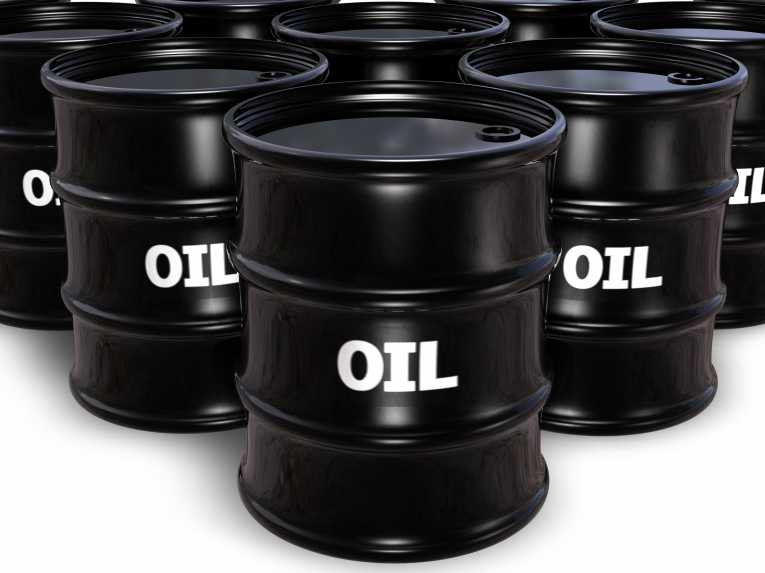
\includegraphics[scale=0.10]{./Chapter1/Figures/figure-oil.jpg}};
\node [anchor=north west] (part1text) at ([xshift=-1em,yshift=0.0em]part1label.south west) {\begin{tabular}{l}{\color{red}{资源}}:可以使机器翻译\\系统运行的``汽油''\end{tabular}};
\end{scope}
}

{
\begin{scope}[yshift=-1.0in,xshift=2.8in]
\node [] (part2label) at (0,0) {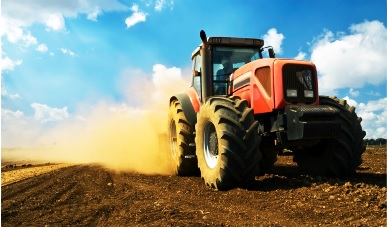
\includegraphics[scale=0.33]{./Chapter1/Figures/figure-truck.jpg}};
\node [anchor=north west] (part2text) at ([xshift=-1em,yshift=0em]part2label.south west) {\begin{tabular}{l}{\color{red}{系统}}:利用资源完成\\自动翻译的程序\end{tabular}};
\end{scope}
}

{
\draw[<-,thick] (part1label.north)..controls +(north:0.6) and +(south:0.6)..([yshift=0.2em]part1.south);
}

{
\draw[<-,thick] ([yshift=0.0em]part2label.north)..controls +(north:0.6) and +(south:0.6)..([yshift=0.2em]part2.south);
}

\end{tikzpicture}



    \caption{机器翻译系统的组成}
    \label{fig:1-2}
\end{figure}
%-------------------------------------------

\parinterval 用机器进行翻译的想法可以追溯到电子计算机产生之前,发展过程中也经历了多个范式的变迁,现代机器翻译系统大多是基于数据驱动的方法\ \dash\ 从数据中自动学习翻译知识,并运用这些知识对新的文本进行翻译。如图\ref{fig:1-2}所示,机器翻译系统通常由两部分组成:

\begin{itemize}
\vspace{0.5em}
\item {\small\bfnew{资源}}:如果把机器翻译系统比作一辆汽车,资源就好比是可以使汽车运行的``汽油'',它包括很多内容,如翻译规则、双(单)语数据、知识库等翻译知识,且这些``知识''都是计算机可读的。值得一提的是,如果没有翻译资源的支持,任何机器翻译系统都无法运行起来。
\vspace{0.5em}
\item {\small\bfnew{系统}}:机器翻译算法的程序实现被称作系统,也就是机器翻译研究人员开发的软件。无论是翻译规则、翻译模板还是统计模型中的参数都需要通过机器翻译系统进行读取和使用。
\vspace{0.5em}
\end{itemize}

\parinterval 构建一个强大的机器翻译系统需要``资源''和``系统''两方面共同作用。在资源方面,随着语料库语言学的发展,已经有大量高质量的双语和单语数据(称为语料)被整理并且电子化存储,研发机器翻译系统所需要的语料基础已经具备。特别是像英语、汉语等世界主流语种,相关语料资源已经非常丰富,这也大大加速了相关研究的进展。当然,对于一些稀缺资源语种或者特殊的领域,语料库仍然匮乏,但是这些并不影响机器翻译领域整体的发展速度。在现有语料库的基础上,很多研究者可以把精力集中在``系统''上。但是,机器翻译并非易事,有以下几方面挑战:

\begin{itemize}
\vspace{0.5em}
\item {\small\bfnew{自然语言翻译问题的复杂性极高}}。语言是人类进化的最高成就之一,自然语言具有高度的概括性、灵活性、多样性,这些都很难用几个简单的模型和算法进行描述。因此,翻译问题的数学建模和计算机程序实现难度很大。虽然近几年Alpha Go等人工智能系统在围棋等领域取得了令人瞩目的成绩,但是,相比翻译来说,围棋等棋类任务仍然``简单'',比如,对于一个句子,其潜在的译文几乎是不可穷尽的,即使同一句话不同人的理解也不尽相同,甚至在翻译一个句子、一个单词的时候,要考虑整个篇章的上下文语境,这些问题都不是传统棋类任务所具备的。
\vspace{0.5em}
\item {\small\bfnew{计算机的``理解''与人类的``理解''存在鸿沟}}。人类一直希望把自己翻译时所使用的知识描述出来,并用计算机程序进行实现,例如早期基于规则的机器翻译方法就源自这个思想。但是,经过实践发现,人和计算机在``理解''自然语言上存在着明显差异。首先,人类的语言能力是经过长时间在多种外部环境因素共同作用下形成的,这种能力很难直接准确地表达。况且人类的语言知识本身就很难描述,更不用说让计算机来理解;其次,人和机器翻译系统理解语言的目的不一样。人理解和使用语言是为了进行生活和工作,而机器翻译系统更多的是为了对某些数学上定义的目标函数进行优化。也就是说,机器翻译系统关注的是翻译这个单一目标,而并不是像人一样进行复杂的活动;此外,人和计算机的运行方式有着本质区别。人类语言能力的生物学机理与机器翻译系统所使用的计算模型本质上是不同的,机器翻译系统使用的是其自身能够理解的``知识'',比如,统计学上的词语表示。这种``知识''并不需要人来理解,当然从系统开发的角度,计算机也并不需要理解人是如何思考的。
\vspace{0.5em}
\item {\small\bfnew{单一的方法无法解决多样的翻译问题}}。首先,语种的多样性会导致任意两种语言之间的翻译实际上都是不同的翻译任务。比如,世界上存在的语言多达几千种,如果选择任意两种语言进行互译就产生上百万种翻译方向。虽然已经有研究者尝试用同一个框架甚至同一个翻译系统进行全语种的翻译,但是这类系统离真正可用还有很远的距离;其次,不同的领域,不同的应用场景对翻译也有不同的需求。比如,文学作品的翻译和新闻的翻译就有不同、口译和笔译也有不同,类似的情况不胜枚举。机器翻译要适用于多样的需求,这些又进一步增加了计算机建模的难度;再次,对于机器翻译来说,充足的高质量数据是必要的,但是不同语种、不同领域、不同应用场景所拥有的数据量有明显差异,甚至很多语种几乎没有可用的数据,这时开发机器翻译系统的难度可想而知。值得注意的是,现在的机器翻译还无法像人类一样在学习少量样例的情况下进行举一反三,因此数据稀缺情况下的机器翻译也给研究者带来了很大的挑战。
\vspace{0.5em}
\end{itemize}


\parinterval 显然,实现机器翻译并不简单,甚至有人把机器翻译看作是实现人工智能的终极目标。幸运的是,今天的机器翻译无论从技术方法上还是从应用上都有了巨大的飞跃,很多问题在不断被求解。如果你看到过十年前机器翻译的结果,再对比今天的结果,一定会感叹翻译质量的今非昔比,很多译文已经非常准确且流畅。从当今机器翻译的前沿技术看,近三十年机器翻译的进步更多的得益于基于数据驱动方法和统计建模方法的使用。特别是近些年深度学习等基于表示学习的端到端方法使得机器翻译的水平达到了新高度。因此,本书将会对基于统计建模和深度学习方法的机器翻译模型、方法和系统实现进行全面介绍和分析,希望这些内容可以对相关内容的学习和科研工作提供参考。

%----------------------------------------------------------------------------------------
%    NEW SECTION
%----------------------------------------------------------------------------------------

\sectionnewpage
\section{机器翻译简史}

\parinterval 虽然翻译这个概念在人类历史中已经存在了上千年,但机器翻译发展至今只有七十余年的历史。纵观机器翻译的发展,历程曲折又耐人寻味,可以说了解机器翻译的历史对我们深入理解相关技术方法会有很好的启发,甚至对我们了解整个自然语言处理领域的发展也有启示作用。

%----------------------------------------------------------------------------------------
%    NEW SUB-SECTION
%----------------------------------------------------------------------------------------

\subsection{人工翻译}

\parinterval 人类形成语言文字的过程中逐渐形成了翻译的概念。一个著名的标志性证据是罗塞塔石碑(Rosetta Stone),如图\ref{fig:1-3}所示。这个石碑制作于公元前196年,据说是可供考证的最久远的记载平行文字的历史遗迹。石碑由上至下刻有同一段埃及国王诏书的三种语言版本,最上面是古埃及象形文,中间是埃及草书,最下面是古希腊文。可以明显看出石碑上中下雕刻的文字的纹理是不同的。尽管用不同的语言文字描述同一件事在今天看来很常见,但是这在生产力低下的两千年前是很罕见的。很多人认为罗塞塔石碑是标志翻译或人工翻译的一个起点。目前罗塞塔石碑保存于大英博物馆,并成为该馆最具代表性的镇馆之宝之一。

%----------------------------------------------
\begin{figure}[htp]
    \centering
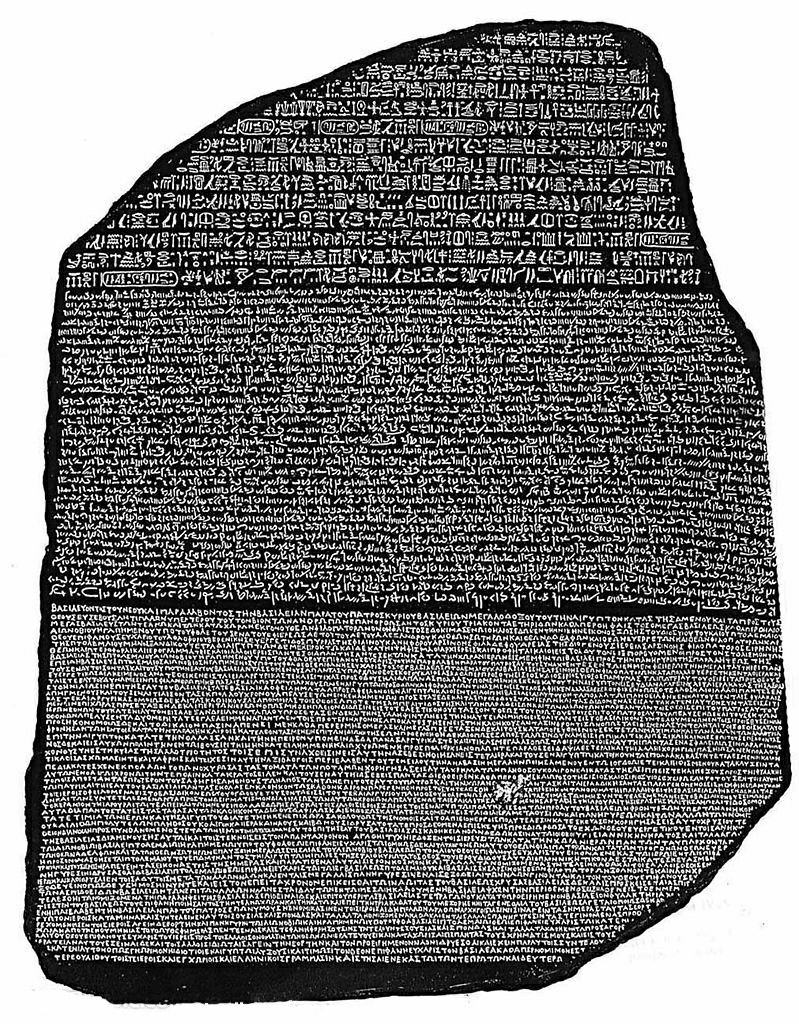
\includegraphics[scale=0.20]{./Chapter1/Figures/figure-rosetta-stone.jpg}
    \caption{罗塞塔石碑}
    \label{fig:1-3}
\end{figure}
%------------------------------------------

\parinterval 随后,更多的翻译工作在文化和知识传播中开展。其中一个典型代表是宗教文献的翻译。在人类的历史长河中,宗教是人类意识形态的一个重要载体。为了宣传教义,人们编写了大量的宗教文献。在西方,一项最早被记录的翻译活动是将旧约圣经(希伯来文及埃兰文)翻译为希腊文版本。迄今为止人类历史上翻译版本最多的书就是圣经。在中国唐代,有一位世界性的重量级文化人物\ \dash \ 玄奘,他不仅是佛学家、旅行家,还是翻译家。玄奘西行求法归来后把全部的心血和智慧奉献给了译经事业,在助手们的帮助下,共翻译佛教经论74部,1335卷,每卷万字左右,合计1335万字,占去整个唐代译经总数的一半以上,树立了我国古代翻译思想的光辉典范。

\parinterval 翻译在人类历史长河中起到了重要的作用。一方面,由于语言文字、文化和地理位置的差异性,使得翻译成为一个重要的需求;另一方面,翻译也加速了不同文明的融会贯通,促进了世界的发展。今天,翻译已经成为重要的行业之一,包括各个高校也都设立了翻译及相关专业,相关人才不断涌现。据《2019年中国语言服务行业发展报告》统计:全球语言服务产值预计将首次接近500亿美元;中国涉及语言服务的在营企业360,000余家,语言服务为主营业务的在营企业近万家,总产值超过300亿元,年增长3\%以上;全国开设外语类专业的高校数量多达上千所,其中设立有翻译硕士(MTI)和翻译本科(BTI)专业的院校分别有250余所和280余所,MTI累计招生数达6万余人\cite{赵军峰2019深化改革}。当然,面对着巨大的需求,如何使用技术手段提高人工翻译效率,比如:机器辅助翻译,也是人工翻译和机器翻译领域需要共同探索的方向。

%----------------------------------------------------------------------------------------
%    NEW SUB-SECTION
%----------------------------------------------------------------------------------------

\subsection{机器翻译的萌芽}

\parinterval 人工翻译已经存在了上千年,而机器翻译又起源于什么时候呢?机器翻译的兴起与发展可以说充满了跌宕起伏,整个发展史可以分为萌芽期、受挫期、快速成长期和爆发期四个阶段。

%----------------------------------------------
\begin{figure}[htp]
    \centering
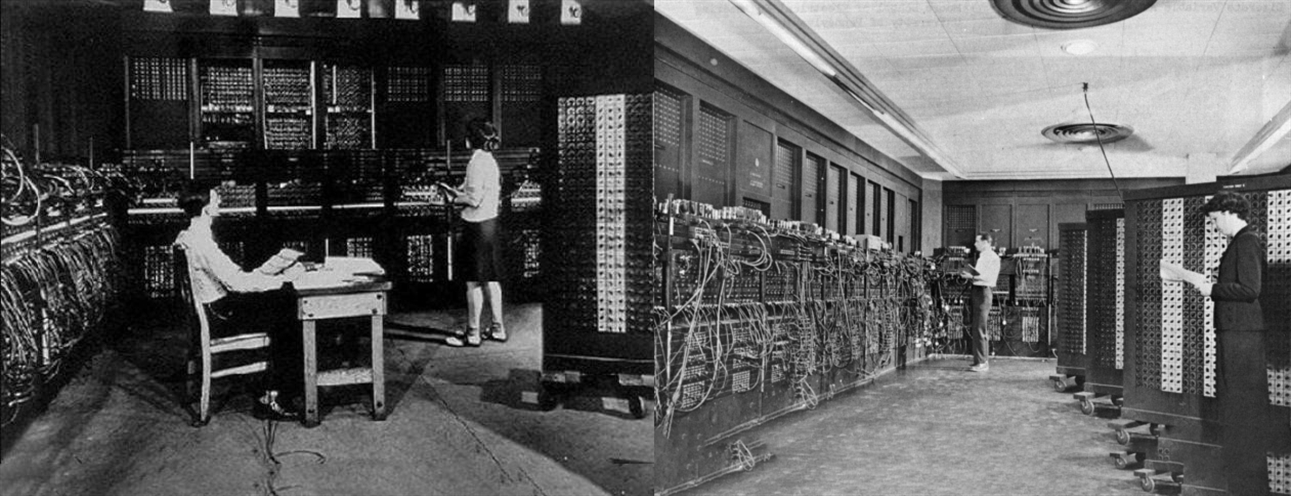
\includegraphics[scale=0.25]{./Chapter1/Figures/figure-eniac.jpg}
    \caption{世界上第一台通用电子数字计算机``埃尼阿克''(ENIAC)}%\\【图片来源:百度百科】
    \label{fig:1-4}
\end{figure}
%-------------------------------------------

\parinterval 世界上第一台通用电子数字计算机在1946年研制成功(图\ref{fig:1-4})。但在上世纪30年代使用计算模型进行自动翻译的思想就开始萌芽,当时法国科学家G.B. Artsouni提出了用机器来进行翻译的想法。

\parinterval 第二次世界大战使得数学和密码学相当发达,由于战争的需要,在那个时代消息传递变的更为隐秘,对文字进行加密和解密成为重要的军事需求。因此,有人提出是否能用密码学的技术或方法解决人类语言的翻译,比如把汉语看成英语的一个加密文本,汉语翻译成英语就类似于解密的过程。当然这只是最初的想法。第一次提出机器翻译这个概念是在1949年,当时W. Weaver撰写了一篇名为《翻译》的备忘录,正式开创了机器翻译(Machine Translation)的概念,这个概念一直沿用至今。当然,在那个年代进行机器翻译研究还有很多条件不具备,包括使用加密解密技术进行自动翻译的很多尝试很快也被验证是不可行的。不过,这些早期的探索为后来机器翻译的发展提供了思想的火种。

%----------------------------------------------------------------------------------------
%    NEW SUB-SECTION
%----------------------------------------------------------------------------------------

\subsection{机器翻译的受挫}

\parinterval 随着电子计算机的发展,研究者开始尝试使用计算机来进行自动的翻译。但是事情并不总是一帆风顺,怀疑论者对机器翻译一直存有质疑,并很容易找出一些机器翻译无法解决的问题。自然地,人们也期望能够客观地评估一下机器翻译的可行性。当时美国基金资助组织委任自动语言处理咨询会承担了这项任务。

\parinterval 经过近两年的调查与分析,该委员会于1966年11月公布了一个题为《语言与机器》的报告(图\ref{fig:1-5}),简称ALPAC报告。该报告全面否定了机器翻译的可行性,为机器翻译的研究泼了一盆冷水。

\parinterval 随后美国政府终止了对机器翻译研究的支持,这导致整个产业界和学术界对机器翻译都开始回避。大家觉得机器翻译像伪科学,无论是发表论文还是申请项目都很难得到支持。没有了政府的支持,企业也无法进行大规模投入,机器翻译的研究就此受挫。

\parinterval 从历史上看,包括机器翻译在内很多人工智能领域在那个年代并不受``待见'',其主要原因在于当时的技术水平还比较低,而大家又对机器翻译等技术的期望过高。最后发现,当时的机器翻译水平无法满足实际需要,因此转而排斥它。但是,也正是这一盆冷水,让人们可以更加冷静的思考机器翻译的发展方向,为后来的爆发蓄力。

%----------------------------------------------
\begin{figure}[htp]
    \centering
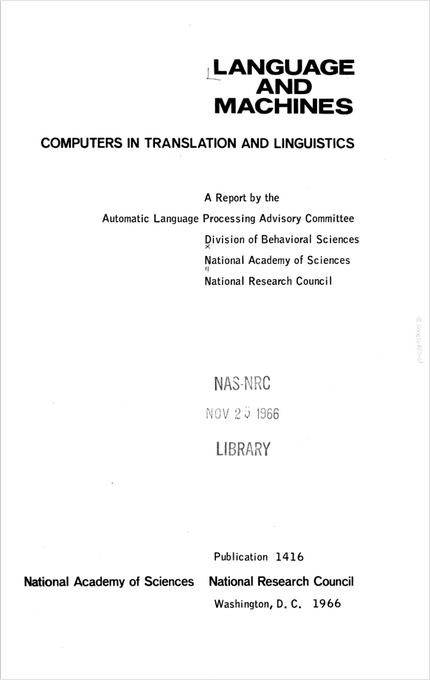
\includegraphics[scale=0.65]{./Chapter1/Figures/figure-report.jpg}
    \caption{ALPAC报告}
    \label{fig:1-5}
\end{figure}
%-------------------------------------------

%----------------------------------------------------------------------------------------
%    NEW SUB-SECTION
%----------------------------------------------------------------------------------------

\subsection{机器翻译的快速成长}

\parinterval 事物发展都是螺旋式上升的,机器翻译也是一样。上世纪70年代中后期,特别是80年代到90年代初,国家之间往来日益密切,而不同语言之间形成的交流障碍愈发严重,传统的人工作业方式已经远远不能满足需求。与此同时,语料库语言学的发展也为机器翻译提供了新的思路。其中,随着传统纸质文字资料不断电子化,计算机可读的语料越来越多,这使得人们可以用计算机对语言规律进行统计分析。另一方面,随着可用数据越来越多,用数学模型描述这些数据中的规律并进行推理逐渐成为可能。这也衍生出一类数学建模方法\ \dash\ {\small\bfnew{数据驱动}}\index{数据驱动}(Data-Driven)\index{Data-Driven}的方法。这类方法也成为了随后出现的统计机器翻译的基础。

传统的机器翻译方法,都需要人来书写规则,虽然对少部分句子具有较高的翻译精度,但这类方法对翻译现象的覆盖度有限,而且对规则或者模板中的噪声非常敏感,系统健壮性差。而基于数据驱动的方法不依赖于人写的规则,机器翻译的建模、训练和推断都可以自动地从数据中学习。这使得整个机器翻译的范式发生了翻天覆地的变化,比如,基于实例的方法和统计机器翻译就是在此期间兴起的。此外,这样的方法使得机器翻译系统的开发代价大大地降低。从上世纪90年代到本世纪初,统计机器翻译发展迅猛,很快成为了当时机器翻译研究与应用的代表性方法。一个标志性的事件是谷歌推出了一个在线的免费自动翻译服务,也就是大家熟知的谷歌翻译。这使得机器翻译这种``高大上''的技术快速进入人们的生活,而不再是束之高阁的科研想法。随着机器翻译不断走向实用,机器翻译的应用也越来越多,这反过来进一步促进了机器翻译的研究进程。比如,在2005-2015年间,统计机器翻译这个主题几乎统治了ACL等自然语言处理相关方向顶级会议的论文,可见其在当时的影响力。

%----------------------------------------------------------------------------------------
%    NEW SUB-SECTION
%----------------------------------------------------------------------------------------

\subsection{机器翻译的爆发}

\parinterval 2005年以后迎来了统计机器翻译发展的十年黄金时期,各种基于统计机器翻译模型层出不穷,经典的基于短语的模型和基于句法的模型也先后被提出。但是在2013年以后,机器学习的进步带来了机器翻译技术的进一步提升。特别是基于神经网络的深度学习方法在机器视觉、语音识别中被成功应用,带来性能的飞跃式提升。很快,相关模型和方法也被用于机器翻译。对于机器翻译来说,深度学习的成功也是一种必然,原因如下:

\begin{itemize}
\vspace{0.5em}
\item 第一,端到端学习不依赖于过多的先验假设。在统计机器翻译时代,模型设计或多或少会对翻译的过程进行假设,称为隐藏结构假设。比如基于短语的模型假设:源语言和目标语言都会被切分成短语序列,这些短语之间存在某种对齐关系。这种假设既有优点也有缺点,一方面,假设可以有助于模型融入人类的先验知识,包括短语本身也借鉴了语言学相关的概念;另一方面,假设越多模型受到的限制也越多。如果假设是正确的,模型可以很好地描述问题。但如果假设错误,那么模型就可能产生偏差。深度学习不依赖于先验知识,也不需要手工设计特征,模型直接从输入和输出的映射上进行学习(端到端学习),这样也在一定程度上避免了隐藏结构假设造成的偏差。
\vspace{0.5em}
\item 第二,神经网络的连续空间模型有更强的表示能力。机器翻译中的一个基本问题是:如何表示一个句子?统计机器翻译把句子的生成过程看作是短语或者规则的推导,这本质上是一个离散空间上的符号系统。深度学习把传统的基于离散化的表示变成了连续空间的表示。比如,用实数空间的分布式表示代替了离散化的词语表示,而整个句子可以被描述为一个实数向量。这使得翻译问题可以在连续空间上描述,进而大大缓解了传统离散空间模型维度灾难等问题。更重要的是,连续空间模型可以用梯度下降等方法进行优化,具有很好的数学性质并且易于实现。
\vspace{0.5em}
\item 第三,深度网络学习算法的发展和GPU(Graphics Processing Unit)等并行计算设备为训练神经网络提供了可能。早期的基于神经网络的方法一直没有在机器翻译甚至自然语言处理领域得到大规模应用,其中一个重要的原因是这类方法需要大量的浮点运算,而且以前计算机的计算能力无法达到这个要求。随着GPU等并行计算设备的进步,训练大规模神经网络也变为了可能。现在已经可以在几亿、几十亿,甚至上百亿句对上训练机器翻译系统,系统研发的周期越来越短,进展日新月异。
\vspace{0.5em}
\end{itemize}

\parinterval 今天,神经机器翻译已经成为新的范式,大有全面替代统计机器翻译之势。比如,从世界上著名的机器翻译比赛WMT和CCMT中就可以看出这个趋势。如图\ref{fig:1-6}所示,其中左图是WMT19全球机器翻译比赛的参赛队伍的截图,这些参赛队伍基本上都在使用深度学习完成机器翻译的建模。而在WMT19各个项目夺冠系统中(\ref{fig:1-6}右图),神经机器翻译也几乎一统天下。

\parinterval 值得一提的是,近些年神经机器翻译的快速发展也得益于产业界的关注。各大互联网企业和机器翻译技术研发机构都对神经机器翻译的模型和实践方法给予了很大贡献。比如,谷歌,微软、百度、搜狗、金山、腾讯、阿里、有道、小牛翻译等企业凭借自身人才和基础设施方面的优势,先后推出了以神经机器翻译为内核的产品及服务,相关技术方法已经在大规模应用中得到验证,大大推动了机器翻译的产业化进程,而且这种趋势在不断加强,机器翻译的前景也更加宽广。

%----------------------------------------------
\begin{figure}[htp]
    \centering
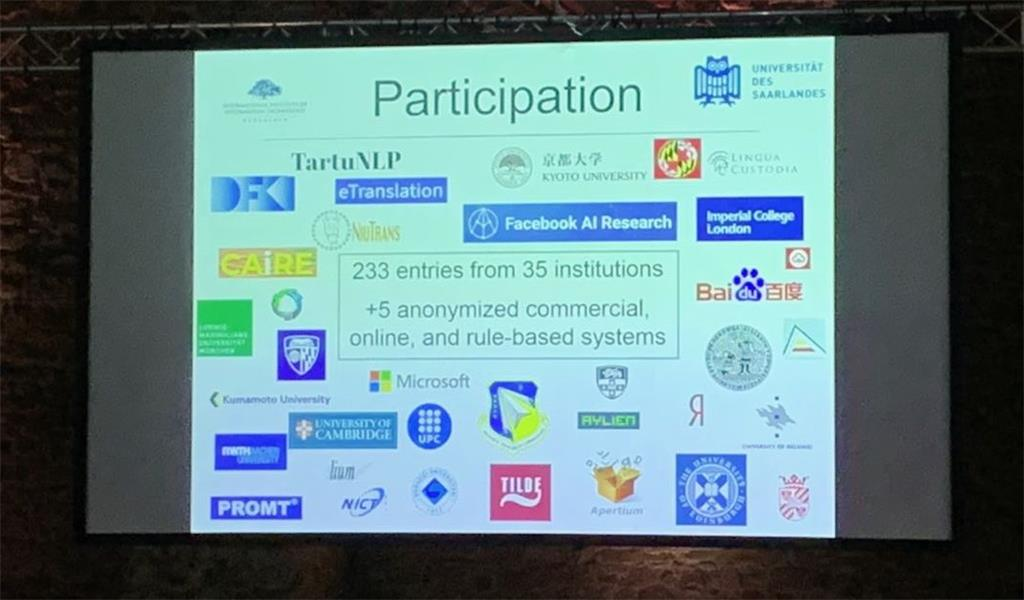
\includegraphics[scale=0.3]{./Chapter1/Figures/figure-wmt-participation.jpg}
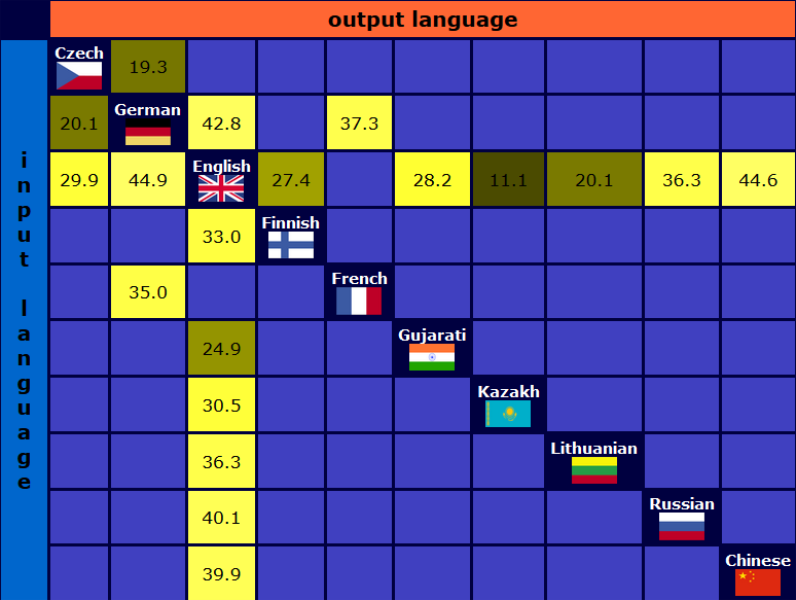
\includegraphics[scale=0.3]{./Chapter1/Figures/figure-wmt-bestresults.jpg}
\setlength{\belowcaptionskip}{-1.5em}
    \caption{国际机器翻译大赛(左:WMT19参赛队伍;右:WMT19最终个项目最好分数结果)}
    \label{fig:1-6}
\end{figure}
%-------------------------------------------

%----------------------------------------------------------------------------------------
%    NEW SECTION
%----------------------------------------------------------------------------------------

\sectionnewpage
\section{机器翻译现状}
%%%%%%%%%%%%%%%%%%%%%%%%%%%%%%%%%%%%%%%%%%%%%%%%%%%%%%%%%%%%%%%%%%%%%%%%%%%%
\parinterval 机器翻译技术发展到今天已经过无数次迭代,技术范式也经过若干次更替,近些年机器翻译的应用也如雨后春笋。但是大家都很好奇今天的机器翻译的质量究竟如何呢?乐观地说,在受限条件下,机器翻译的译文结果还是非常不错的,甚至可以接近人工翻译的结果。然而,在开放式翻译任务中,机器翻译的结果却并不理想。更严格来说,机器翻译的质量远没有达到人们所期望的完美的程度。对于有些人提到的``机器翻译代替人工翻译''也并不是事实。比如,在高精度同声传译任务中,机器翻译仍需要更多打磨;再比如,针对于小说的翻译,机器翻译还无法做到与人工翻译媲美;甚至有人尝试用机器翻译系统翻译中国古代诗词,这里更多的是娱乐的味道。但是毫无疑问的是,机器翻译可以帮助人类,甚至有朝一日可以代替一些低端的人工翻译工作。

\parinterval 图\ref{fig:1-7}展示了机器翻译和人工翻译质量的一个对比结果。在汉语到英语的新闻翻译任务中,如果对译文进行人工评价,五分制机器翻译的译文得3.9 分,人工译文得4.7分(人的翻译也不是完美的)。可见,在这个任务中机器翻译表现不错,但是与人还有一定差距。如果换一种方式评价,把人的译文作为参考答案,用机器翻译的译文与其进行比对,会发现机器翻译的得分只有47分(百分制)。当然,这个结果并不是说机器翻译的译文质量很差,它更多的是表明机器翻译系统可以生成一些与人工翻译不同的译文,机器翻译也具有一定的创造性。这也类似于,很多围棋选手都想向AlphaGo学习,因为智能围棋系统也可以走出一些人类从未走过的妙招。

%----------------------------------------------
\begin{figure}[htp]
   \centering

\definecolor{ublue}{rgb}{0.152,0.250,0.545}
\definecolor{ugreen}{rgb}{0,0.5,0}


%%% outline
%-------------------------------------------------------------------------

{
\begin{tikzpicture}
\node [anchor=south west, fill=blue!50, minimum width=1.1cm, minimum height=2.3cm] (mt) at (1,0) {{\color{white} {\small\sffamily\bfseries{机器}}}};
\node [anchor=south west, fill=red!50, minimum width=1.1cm, minimum height=2.7cm] (human) at ([xshift=0.5cm]mt.south east) {{\color{white} {\small\sffamily\bfseries{人}}}};
\node [anchor=south] (mtscore) at (mt.north) {3.9};
\node [anchor=south] (humanscore) at (human.north) {4.7};
\draw [->,thick] ([xshift=-0.5cm]mt.south west) -- ([xshift=0.5cm]human.south east);
\draw [->,thick] ([xshift=-0.5cm]mt.south west) -- ([xshift=-0.5cm,yshift=3.2cm]mt.south west);

\node [anchor=south west, fill=blue!50, minimum width=1.1cm, minimum height=1.5cm] (mt1) at ([xshift=13.0em,yshift=-3.0em]mt.east) {{\color{white} {\small\sffamily\bfseries{机器}}}};
\node [anchor=south west, fill=red!50, minimum width=1.1cm, minimum height=2.7cm] (human1) at ([xshift=0.5cm]mt1.south east) {{\color{white} {\small\sffamily\bfseries{人}}}};
\node [anchor=south] (mtscore1) at (mt1.north) {47};
\node [anchor=south] (humanscore1) at (human1.north) {100};
\draw [->,thick] ([xshift=-0.5cm]mt1.south west) -- ([xshift=0.5cm]human1.south east);
\draw [->,thick] ([xshift=-0.5cm]mt1.south west) -- ([xshift=-0.5cm,yshift=3.2cm]mt1.south west);

\node[anchor=south](footname1) at ([xshift=2.1em,yshift=-2.0em]mt.south){\footnotesize{人工评价(五分制)}};
\node[anchor=south](footname2) at ([xshift=2.1em,yshift=-2.0em]mt1.south){\footnotesize{自动评价(百分制)}};
\end{tikzpicture}

}






%---------------------------------------------------------------------




\setlength{\belowcaptionskip}{-0.5em}
    \caption{机器翻译与人工翻译性能对比(汉英新闻领域翻译)}
    \label{fig:1-7}
\end{figure}
%-------------------------------------------

\parinterval 图\ref{fig:1-9}展示了一个真实的汉语到英语翻译实例。对比发现,机器翻译与人工翻译还是存在差距的,特别是在翻译一些具有感情色彩的词语时,机器翻译的译文缺一些味道。那么,机器翻译一点用都没有吗?显然不是。实际上,如果考虑翻译速度与翻译代价,机器翻译的价值是无可比拟的。还是同一个例子,翻译一篇短文如果人工翻译需要30分钟甚至更长时间,那么机器翻译仅仅需要两秒,换种情况思考,如果有100万篇这样的文档,其人工翻译的成本根本无法想象,消耗的时间更是难以计算,而计算机集群仅仅需要一天,而且只有电力的消耗。
%\\ \\ \\ \\ \\ \\ \\ \\ \\ \\ \\ \\ \\ \\ \\ \\ \\ \\ \\ \\ \\

%----------------------------------------------
\begin{figure}[htp]
    \centering
\definecolor{ublue}{rgb}{0.152,0.250,0.545}
\definecolor{ugreen}{rgb}{0,0.5,0}

%%% outline
%-------------------------------------------------------------------------
\begin{tikzpicture}
%第一段----------------------------------------------
%原文-------------
\node [pos=0.4,left,xshift=-0.4em,yshift=2.0em] (original1) {\scriptsize{源\ \ 语\ \ 言:从前有一个小岛,上面住着快乐、悲哀、知识和爱,还有其他各种情感。一天,情感们得知}};
\node [anchor=north west] (original1-1) at ([xshift=3.5em,yshift=0.3em]original1.south west)  {\scriptsize{小岛快要下沉了。于是,大家都准备船只,离开小岛,只有爱决定留下来,她想坚持到最后}};
\node [anchor=north west] (original1-2) at ([yshift=0.3em]original1-1.south west)  {\scriptsize{一刻。过了几天,小岛真的要下沉了,爱想请人帮忙。}};
%机器翻译--------------
\node [anchor=north west] (mt1) at ([xshift=-3.5em,yshift=0.3em]original1-2.south west) {\scriptsize{机器翻译:Once upon a time there was an island {\color{red}\underline{on which}} lived happiness,sorrow,knowledge,love and other}};

\node [anchor=north west] (mt1-1) at ([xshift=3.5em,yshift=0.4em]mt1.south west) {\scriptsize{emotions. One day, {\color{red}\underline{the}} emotions learned that the island was going to sink.As a result,everyone pre}};

\node [anchor=north west] (mt1-2) at ([yshift=0.4em]mt1-1.south west) {\scriptsize{-pared the boat and {\color{red}\underline{left the island.}} Only Love decided to stay.She {\color{red}\underline{ wanted to stick}} to it until the last}};

\node [anchor=north west] (mt1-3) at ([yshift=0.4em]mt1-2.south west) {\scriptsize{moment. After a few days, the island was really going to sink and love {\color{red}\underline{ wanted help.}}}};
%人工翻译---------------
\node [anchor=north west] (ht1) at ([xshift=-3.5em,yshift=0.4em]mt1-3.south west) {\scriptsize{人工翻译:Once upon a time, there was a small island {\color{red}\underline{where}} lived all kinds of emotions like JOY,SADNESS,}};

\node [anchor=north west] (ht1-1) at ([xshift=3.5em,yshift=0.4em]ht1.south west) {\scriptsize{KNOWLEDGE, and LOVE.One day, {\color{red}\underline{these}} emotions found that the island was sinking, so one by}};

\node [anchor=north west] (ht1-2) at ([yshift=0.4em]ht1-1.south west) {\scriptsize{one they prepared the boat and {\color{red}\underline{planned to leave.}} None but LOVE chose to stay there. She {\color{red}\underline{was deter}}}};

\node [anchor=north west] (ht1-3) at ([yshift=0.4em]ht1-2.south west) {\scriptsize{{\color{red}\underline{-mined to}} persist till the last moment.A few days later, almost the whole island sunk into the sea,}};

\node [anchor=north west] (ht1-4) at ([yshift=0.4em]ht1-3.south west) {\scriptsize{and LOVE had to {\color{red}\underline{seek for help.}}}};

\begin{pgfonlayer}{background}
{
\node[rectangle,draw=ublue, inner sep=0mm] [fit =(original1)(ht1)(mt1)(ht1-4)] {};
}
\end{pgfonlayer}


\end{tikzpicture}





\end{figure}
\begin{figure}[t]
    \centering
\definecolor{ublue}{rgb}{0.152,0.250,0.545}
\definecolor{ugreen}{rgb}{0,0.5,0}

%%% outline
%-------------------------------------------------------------------------
\begin{tikzpicture}
\node [pos=0.4,left,xshift=-0.4em,yshift=2.0em,,opacity=0.0] (original1) {\scriptsize{源 \qquad 文:从前有一个小岛,上面住着快乐、悲哀、知识和爱,还有其他各种情感。一天,情感们得知}};
\node [anchor=north west] (mt4-2) at ([xshift=3.5em,yshift=0.3em]original1.south west) {\scriptsize{ Love saw vanity in a magnificent boat and said, ``Vanity, help me!'' ``I can't help you. You are {\color{red}\underline{soak}}}};
\node [anchor=north west] (mt4-3) at ([yshift=0.4em]mt4-2.south west) {\scriptsize{{\color{red}\underline{-ed to the skin}} and will damage my beautiful boat.'' When sorrow came, love asked him for help: ``}};

\node [anchor=north west] (mt4-4) at ([yshift=0.4em]mt4-3.south west) {\scriptsize{sorrow, let me go with you!'' ``Oh,...love, I am so sad that I want to be alone for a while!'' Sadly rep}};
\node [anchor=north west] (mt4-5) at ([yshift=0.4em]mt4-4.south west) {\scriptsize{-lied. Happiness {\color{red}\underline{approached}} love, but she was too happy to hear love calling her!}};

%人工翻译---------------
\node [anchor=north west] (ht4) at ([xshift=-3.5em,yshift=0.3em]mt4-5.south west) {\scriptsize{人工翻译:At that moment, WEALTH {\color{red}\underline{was passing by}} in a big boat. Love said,``WEALTH, can you take me}};

\node [anchor=north west] (ht4-1) at ([xshift=3.5em,yshift=0.4em]ht4.south west) {\scriptsize{with you?'' WEALTH answered, ``no, {\color{red}\underline{there is a lot}} of gold and silver in my boat. There is no place}};

\node [anchor=north west] (ht4-2) at ([yshift=0.4em]ht4-1.south west) {\scriptsize{for you.'' Love saw VANITY in a beautiful boat and said, ``VANITY, help me!'' ``I can't help you.}};
\node [anchor=north west] (ht4-3) at ([yshift=0.4em]ht4-2.south west) {\scriptsize{You are {\color{red}\underline{all wet,}} and will break my pretty boat.'' Then SADNESS came. Love asked for help,``SAD}};

\node [anchor=north west] (ht4-4) at ([yshift=0.4em]ht4-3.south west) {\scriptsize{-NESS, let me go with you!'' ``Oh,...LOVE, I am so sad that I want to be alone for a while!'' ``Repli}};
\node [anchor=north west] (ht4-5) at ([yshift=0.4em]ht4-4.south west) {\scriptsize{-ed SADNESS. JOY {\color{red}\underline{came close to }} love, but she was so happy that she did not hear him call her!}};

%第三段--------------------------------
\node[anchor=north west] (original8) at ([xshift=-3.5em,yshift=-0.3em]ht4-5.south west)  {\scriptsize{源 \qquad 文:突然,一个声音传来:``过来,爱,我带你走。''这是位长者。爱大喜过望,竟忘了问他他}};
\node[anchor=north west] (original8-1) at ([xshift=3.5em,yshift=0.3em]original8.south west)  {\scriptsize{的名字。登上陆地后,长者独自走开了。爱对长者感激不尽,问另一位长者知识:``帮我的}};
\node[anchor=north west] (original8-2) at ([yshift=0.3em]original8-1.south west)  {\scriptsize{那个人是谁?''``他是时间。''知识老人回答。``时间?''爱问道,``他为什么要帮我?''知识老}};
\node[anchor=north west] (original8-3) at ([yshift=0.3em]original8-2.south west)  {\scriptsize{人笑道:``因为只有时间才能理解爱有多么伟大。''}};
%机器翻译--------------
\node [anchor=north west] (mt8) at ([xshift=-3.5em,yshift=0.4em]original8-3.south west) {\scriptsize{机器翻译:Suddenly, a voice {\color{red}\underline{came:}} ``Come here, love, I'll take you away.'' This is an elder. Love was {\color{red}\underline{overjoy}}}};
\node [anchor=north west] (mt8-1) at ([xshift=3.5em,yshift=0.4em]mt8.south west) {\scriptsize{{\color{red}\underline{-ed and}} forgot to ask his name. After landing on land, the elder walked away alone.Love was very}};
\node [anchor=north west] (mt8-2) at ([yshift=0.4em]mt8-1.south west) {\scriptsize{grateful to the elder and asked another elder knowledge, {\color{red}\underline{``Who is the person who helped me?''}} ``He}};
\node [anchor=north west] (mt8-3) at ([yshift=0.4em]mt8-2.south west) {\scriptsize{is time.'' The {\color{red}\underline{old intellectual}} replied. ``Time?'' Love asked,``Why did he help me?'' The old intellec}};
\node [anchor=north west] (mt8-4) at ([yshift=0.4em]mt8-3.south west) {\scriptsize{-tual laughed, ``Because only time canunderstand how great love is.''}};
%人工翻译---------------
\node [anchor=north west] (ht8) at ([xshift=-3.5em,yshift=0.4em]mt8-4.south west) {\scriptsize{人工翻译:Suddenly, a voice {\color{red}\underline{said,}} ``come, LOVE, I'll take you.'' This is an elder. LOVE was {\color{red}\underline{so over that}} she}};
\node [anchor=north west] (ht8-1) at ([xshift=3.5em,yshift=0.4em]ht8.south west) {\scriptsize{forgot to ask his name. After landing on land, the elder walked away}};
\node [anchor=north west] (ht8-2) at ([yshift=0.4em]ht8-1.south west) {\scriptsize{alone.LOVE was so grateful to the elder that she asked KNOWLEDGE, another elder, {\color{red}\underline{``who help}}}};
\node [anchor=north west] (ht8-3) at ([yshift=0.4em]ht8-2.south west) {\scriptsize{{\color{red}\underline{-ed me?''}} ``He is TIME.'' The {\color{red}\underline{old man}} replied. ``TIME?'' LOVE asked. ``why did he help me?'' The}};
\node [anchor=north west] (ht8-4) at ([yshift=0.4em]ht8-3.south west) {\scriptsize{old man smiled and said, ``Because only time can understand how great love is.''}};

%{
%\draw[dotted,thick,ublue] ([xshift=10.3em,yshift=0.3em]mt8.south west)--%([xshift=-5.2em,yshift=-0.3em]ht8.north);
%}



\begin{pgfonlayer}{background}
{
\node[rectangle,draw=ublue, inner sep=0mm] [fit = (mt4-2)(ht4)(ht8-4)] {};
}
\end{pgfonlayer}


\end{tikzpicture}





    \caption{机器翻译与人工翻译实例结果对比}
\setlength{\belowcaptionskip}{7.0em}
    \label{fig:1-9}
\end{figure}
%-------------------------------------------

%----------------------------------------------------------------------------------------
%    NEW SECTION
%----------------------------------------------------------------------------------------

\sectionnewpage
\section{机器翻译方法}
%%%%%%%%%%%%%%%%%%%%%%%%%%%%%%%%%%%%%%%%%%%%%%%%%%%%%%%%%%%%%%%%%%%%%%%%%%%%
\parinterval 为了对机器翻译技术有一个整体的认识,这里对一些主要的机器翻译框架进行简要介绍。

%----------------------------------------------------------------------------------------
%    NEW SUB-SECTION
%----------------------------------------------------------------------------------------

\subsection{基于规则的机器翻译}

\parinterval 早期的机器翻译研究都是以基于规则的方法为主,特别是在上世纪70年代,以基于规则方法为代表的专家系统是人工智能中最具代表性的研究领域。它的主要思想是以词典和人工书写的规则库作为翻译知识,用一系列规则的组合完成翻译。

\parinterval 图\ref{fig:1-8}展示了一个使用规则进行翻译的实例。这里,利用一个简单的汉译英规则库完成对句子``我对你感到满意''的翻译。当翻译``我''时,从规则库中找到规则1,该规则表示遇到单词``我''就翻译为``I'';类似地,也可以从规则库中找到规则4,该规则表示翻译调序,即将单词``you''放到``be satisfied with''后面。可以看到,这些规则的使用和进行翻译时所使用的思想非常类似,可以说基于规则方法实际上在试图描述人类进行翻译的思维过程。

%----------------------------------------------
\begin{figure}[htp]
    \centering
\definecolor{ublue}{rgb}{0.152,0.250,0.545}
\definecolor{ugreen}{rgb}{0,0.5,0}


%%% outline
%-------------------------------------------------------------------------

\begin{tikzpicture}
\begin{scope}
{
{\footnotesize
\node [anchor=north west] (rule1) at (0,0) {\textbf{1: If} 源=我, \textbf{then} 译=\ I};
\node [anchor=north west] (rule2) at ([yshift=0.1em]rule1.south west) {\textbf{2: If} 源=你, \textbf{then} 译=\ you};
\node [anchor=north west] (rule3) at ([yshift=0.1em]rule2.south west) {\textbf{3: If} 源=感到\ 满意,};
\node [anchor=north west] (rule3part2) at ([yshift=0.5em]rule3.south west) {\textbf{\hspace{0.95em} then} 译=\ be satisfied with};
\node [anchor=north west] (rule4) at ([yshift=0.1em]rule3part2.south west) {\textbf{4: If} 源=对 ... 动词[表态度]};
\node [anchor=north west] (rule4part2) at ([yshift=0.5em]rule4.south west) {\textbf{\hspace{0.95em} then} 调序[动词 + 对象]};
\node [anchor=north west] (rule5) at ([yshift=0.1em]rule4part2.south west) {\textbf{5: If} 译文主语是\ I};
\node [anchor=north west] (rule5part2) at ([yshift=0.5em]rule5.south west) {\textbf{\hspace{0.95em} then} be动词为\ am/was};
\node [anchor=north west] (rule6) at ([yshift=0.1em]rule5part2.south west) {\textbf{6: If} 源语是主谓结构};
\node [anchor=north west] (rule6part2) at ([yshift=0.5em]rule6.south west) {\textbf{\hspace{0.95em} then} 译文为主谓结构};
\node [anchor=south west] (rulebaselabel) at (rule1.north west) {{\color{ublue} 资源:规则库}};
}

\begin{pgfonlayer}{background}
{
  \node[rectangle,draw=ublue, thick,inner sep=0mm] [fit = (rule1) (rule2) (rule3) (rule3part2) (rule4) (rule4part2) (rule5) (rule5part2) (rule6) (rule6part2) (rulebaselabel)] {};
}
\end{pgfonlayer}
}

\end{scope}

\begin{scope}[xshift=2.3in]
{\footnotesize
\node [anchor=north west,inner sep=1mm] (w1) at (0,0em) {我};
\node [anchor=north west,inner sep=1mm] (w2) at ([xshift=0.3em]w1.north east) {对};
\node [anchor=north west,inner sep=1mm] (w3) at ([xshift=0.3em]w2.north east) {你};
\node [anchor=north west,inner sep=1mm] (w4) at ([xshift=0.3em]w3.north east) {感到};
\node [anchor=north west,inner sep=1mm] (w5) at ([xshift=0.3em]w4.north east) {满意};
}
\end{scope}

{\footnotesize
\node [anchor=north,inner sep=1mm] (t1) at ([yshift=-0.6em]w1.south) {I};
\draw[->,thick,ublue] (w1.south)--(t1.north);
}

{\footnotesize
\node [anchor=north,inner sep=1mm] (t3) at ([yshift=-0.6em]w3.south) {you};
\draw[->,thick,ublue] (w3.south)--(t3.north);
}

{\footnotesize
\draw[-] ([yshift=0.2em]w4.south west)--([yshift=0.2em]w5.south east);
\node [anchor=north,inner sep=1mm] (t45) at ([yshift=-2em]w5.south) {be satisfied with};
\draw[->,thick,ublue] ([yshift=0.1em]w4.south east)..controls +(south:0.6) and +(north:0.6)..(t45.north);
}

{\footnotesize
\node [anchor=north west,inner sep=1mm] (t35) at ([yshift=-3.0em,xshift=-1em]t3.south) {be satisfied with you};
\draw[->,thick,ublue] (t3.south)..controls +(south:1.3) and +(north:0.9)..([xshift=-1em,yshift=-0.2em]t35.north east);
\draw[->,thick,ublue] (t45.south)..controls +(south:0.7) and +(north:0.5)..([xshift=3em,yshift=-0.2em]t35.north west);
}

{\footnotesize
\node [anchor=north west,inner sep=1mm] (t15) at ([yshift=-1.5em,xshift=-2em]t35.south west) {I be satisfied with you};
\draw[->,thick,ublue] (t35.south)..controls +(south:0.5) and +(north:0.5)..([xshift=-5em]t15.north east);
\draw[->,thick,ublue] (t1.south)..controls +(south:1.5) and +(north:1.5)..([xshift=0.5em]t15.north west);
}


{\footnotesize
\node [anchor=north west,inner sep=1mm] (t15final) at ([yshift=-1.5em]t15.south west) {I am satisfied with you};
\node [draw,circle,thick,dotted,ublue,minimum width=1.3em] (be1) at ([xshift=1.35em,yshift=0.1em]t15.west) {};
\draw[->,thick,ublue] ([xshift=-0em]be1.south)..controls +(south:0.3) and +(north:0.4)..([xshift=1.6em,yshift=-0.2em]t15final.north west);
}
{
\draw[->,dotted,thick,red] ([xshift=-0.2em]rule5part2.east)..controls +(east:1.5) and +( west:1.5)..(t15final.west) node[pos=0.9,below,xshift=0.3em,yshift=0.0em] (applyr6) {\color{red}{\tiny\sffamily\bfseries{规则5}}};
}

\end{tikzpicture}
%---------------------------------------------------------------------



\setlength{\belowcaptionskip}{-1.5em}
    \caption{基于规则的机器翻译的示例图(左:规则库;右:规则匹配结果)}
    \label{fig:1-8}
\end{figure}
%-------------------------------------------

\parinterval 但是,基于规则的机器翻译也存在问题。首先,书写规则需要消耗大量人力,规则库的维护代价极高;其次,规则很难涵盖所有的语言现象;再有,自然语言存在大量的歧义现象,规则之间也会存在冲突,这也导致规则数量不可能无限制增长。

%----------------------------------------------------------------------------------------
%    NEW SUB-SECTION
%----------------------------------------------------------------------------------------

\subsection{基于实例的机器翻译}

\parinterval 基于规则的方法更多地被使用在受限翻译场景中,比如受限词汇集的翻译。针对基于规则的方法存在的问题,基于实例的机器翻译于上世纪80年代中期被提出\cite{nagao1984framework}。该方法的基本思想是在双语句库中找到与待翻译句子相似的实例,之后对实例的译文进行修改,如替换、增加、删除等一系列操作,从而得到最终译文。这个过程可以类比人类学习并运用语言的过程:人会先学习一些翻译实例或者模板,当遇到新的句子时,会用以前的实例和模板作对比,之后得到新的句子的翻译结果。这也是一种举一反三的思想。

%----------------------------------------------
\begin{figure}[htp]
    \centering

\definecolor{ublue}{rgb}{0.152,0.250,0.545}
\definecolor{ugreen}{rgb}{0,0.5,0}


%%% outline
%-------------------------------------------------------------------------

\begin{tikzpicture}
\begin{scope}
{
{\footnotesize
\node [anchor=north west] (example1) at (0,0) {\textbf{1:} 源=什么\ 时候\ 开始};
\node [anchor=north west] (example1part2) at ([yshift=0.5em]example1.south west) {\hspace{1em} 译=\ When will it start};
\node [anchor=north west] (example2) at ([yshift=0.1em]example1part2.south west) {\textbf{2:} 源=我\ 对\ 他\ 感到\ 高兴};
\node [anchor=north west] (example2part2) at ([yshift=0.5em]example2.south west) {\hspace{1em} 译=\ I am happy with him};
\node [anchor=north west] (example3) at ([yshift=0.1em]example2part2.south west) {\hspace{1em} ...};
\node [anchor=south west] (examplebaselabel) at (example1.north west) {{\color{ublue} 资源1:翻译实例库}};
}
}

\begin{pgfonlayer}{background}
{
\node[rectangle,draw=ublue, inner sep=0mm] [fit = (example1) (example1part2) (example2) (example2part2) (example3) (examplebaselabel)] {};
}
\end{pgfonlayer}

\end{scope}

\begin{scope} [yshift=-1.3in]
{\footnotesize
{
\node [anchor=north west] (entry1) at (0,0) {\textbf{1:} 我 $\to$ I $\mid$ me};
\node [anchor=north west] (entry2) at ([yshift=0.1em]entry1.south west) {\textbf{2:} 你 $\to$ you};
\node [anchor=north west] (entry3) at ([yshift=0.1em]entry2.south west) {\textbf{3:} 满意 \hspace{-0.4em} $\to$ \hspace{-0.4em} satisfy \hspace{-0.12em}$\mid$\hspace{-0.12em} satisfied ... };
\node [anchor=north west] (entry4) at ([yshift=0.1em]entry3.south west) {\hspace{1em} ...};
\node [anchor=south west] (dictionarylabel) at (entry1.north west) {{\color{ublue} 资源2:翻译词典}};
}
}

\begin{pgfonlayer}{background}
{
\node[rectangle,draw=ublue, inner sep=0mm] [fit = (entry1) (entry2) (entry3) (entry4) (dictionarylabel)] {};
}
\end{pgfonlayer}

\end{scope}

\begin{scope}[xshift=2.3in]
{\footnotesize
\node [anchor=north west,inner sep=1mm] (w1) at (0,1.7em) {我};
\node [anchor=north west,inner sep=1mm] (w2) at ([xshift=0.3em]w1.north east) {对};
\node [anchor=north west,inner sep=1mm] (w3) at ([xshift=0.3em]w2.north east) {你};
\node [anchor=north west,inner sep=1mm] (w4) at ([xshift=0.3em]w3.north east) {感到};
\node [anchor=north west,inner sep=1mm] (w5) at ([xshift=0.3em]w4.north east) {满意};
}
\end{scope}

\begin{scope}[xshift=2.3in,yshift=-0.2in]
{\footnotesize
\node [anchor=north west,inner sep=1mm] (c1) at (0,0) {我};
\node [anchor=north west,inner sep=1mm] (c2) at ([xshift=0.3em]c1.north east) {对};
\node [anchor=north west,inner sep=1mm] (c3) at ([xshift=0.3em]c2.north east) {他};
\node [anchor=north west,inner sep=1mm] (c4) at ([xshift=0.3em]c3.north east) {感到};
\node [anchor=north west,inner sep=1mm] (c5) at ([xshift=0.3em]c4.north east) {高兴};
}
\end{scope}

\begin{scope}[xshift=2.3in,yshift=-0.6in]
{\footnotesize
\node [anchor=west,inner sep=1mm] (e1) at (0,0) {I};
\node [anchor=west,inner sep=1mm] (e2) at ([xshift=0.3em]e1.east) {am};
\node [anchor=west,inner sep=1mm] (e3) at ([xshift=0.3em]e2.east) {happy};
\node [anchor=west,inner sep=1mm] (e4) at ([xshift=0.3em]e3.east) {with};
\node [anchor=west,inner sep=1mm] (e5) at ([xshift=0.3em]e4.east) {him};
}
\end{scope}

{
\draw[<->,dotted,thick,red] (example2.east)..controls +(east:0.6) and +(west:0.6)..(c1.west) node[pos=0.9,left,xshift=0.6em,yshift=0.4em] (simexample) {\color{red}{\tiny{相似实例}}};
\draw[<->,dotted,thick,red] ([xshift=-0.2em]example2part2.east)..controls +(east:0.5) and +(west:0.5)..(e1.west);
}

{
\draw[<->,dotted,thick,ublue] (w3.south)--(c3.north) node[pos=0.5,right] (mismatch1) {\color{red}{\tiny{不匹配}}};
\draw[dotted,thick,ublue] ([xshift=-0.6em,yshift=0.0em]c3.south east)--([xshift=0.8em,yshift=0.0em]e5.north west);
}

{
\draw[<->,dotted,thick,ublue] (w5.south)--(c5.north) node[pos=0.5,right] (mismatch1) {\color{red}{\tiny{不匹配}}};
\draw[dotted,thick,ublue] ([xshift=0.8em,yshift=0.0em]c5.south west)--([xshift=0.0em,yshift=-0.2em]e3.north);
}

{
\draw[double,->,thick,ublue] (e3.south)--([yshift=-1.2em]e3.south) node[pos=0.5,right,xshift=0.2em,yshift=0.2em] (step1) {\color{red}{\tiny{用“你”替换“他”}}};

\draw[->,dotted,thick,red] ([xshift=-0.1em]entry2.east)..controls +(east:4) and +(west:4)..([yshift=-0.6em,xshift=-0.5em]e3.south) ;
}

\begin{scope}[xshift=2.3in,yshift=-0.9in]
{\footnotesize
\node [anchor=north west,inner sep=1mm] (c1) at (0,0) {我};
\node [anchor=north west,inner sep=1mm] (c2) at ([xshift=0.3em]c1.north east) {对};
\node [anchor=north west,inner sep=1mm] (c3) at ([xshift=0.3em]c2.north east) {\footnotesize{{\color{ublue} 你}}};
\node [anchor=north west,inner sep=1mm] (c4) at ([xshift=0.3em]c3.north east) {感到};
\node [anchor=north west,inner sep=1mm] (c5) at ([xshift=0.3em]c4.north east) {高兴};
}
\end{scope}

\begin{scope}[xshift=2.3in,yshift=-1.3in]
{\footnotesize
\node [anchor=west,inner sep=1mm] (e1) at (0,0) {I};
\node [anchor=west,inner sep=1mm] (e2) at ([xshift=0.3em]e1.east) {am};
\node [anchor=west,inner sep=1mm] (e3) at ([xshift=0.3em]e2.east) {happy};
\node [anchor=west,inner sep=1mm] (e4) at ([xshift=0.3em]e3.east) {with};
\node [anchor=west,inner sep=1mm] (e5) at ([xshift=0.3em,yshift=-0.2em]e4.east) {\textbf{{\color{ublue} you}}};
}
\end{scope}

{
\draw[dotted,thick,ublue] ([xshift=-0.6em,yshift=0.0em]c3.south east)--([xshift=0.8em,yshift=0.0em]e5.north west);
}

{
\draw[double,->,thick,ublue] (e3.south)--([yshift=-1.2em]e3.south) node[pos=0.5,right,xshift=0.2em,yshift=0.2em] (step1) {\color{red}{\tiny{用“满意”替换“高兴”}}};

\draw[->,dotted,thick,red] ([xshift=-1.2em,yshift=-0.6em]entry3.north east)..controls +(east:2) and +(west:3)..([yshift=-0.6em,xshift=-0.5em]e3.south) ;
}

\begin{scope}[xshift=2.3in,yshift=-1.6in]
{\footnotesize
\node [anchor=north west,inner sep=1mm] (c1) at (0,0) {我};
\node [anchor=north west,inner sep=1mm] (c2) at ([xshift=0.3em]c1.north east) {对};
\node [anchor=north west,inner sep=1mm] (c3) at ([xshift=0.3em]c2.north east) {你};
\node [anchor=north west,inner sep=1mm] (c4) at ([xshift=0.3em]c3.north east) {感到};
\node [anchor=north west,inner sep=1mm] (c5) at ([xshift=0.3em]c4.north east) {\footnotesize{{\color{ublue} 满意}}};
}
\end{scope}

\begin{scope}[xshift=2.3in,yshift=-2.0in]
{\footnotesize
\node [anchor=west,inner sep=1mm] (e1) at (0,0) {I};
\node [anchor=west,inner sep=1mm] (e2) at ([xshift=0.3em]e1.east) {am};
\node [anchor=west,inner sep=1mm] (e3) at ([xshift=0.3em]e2.east) {\textbf{{\color{ublue} satisfied}}};
\node [anchor=west,inner sep=1mm] (e4) at ([xshift=0.3em]e3.east) {with};
\node [anchor=west,inner sep=1mm] (e5) at ([xshift=0.3em,yshift=-0.2em]e4.east) {you};
}
\end{scope}

{
\draw[dotted,thick,ublue] ([xshift=1.0em,yshift=0.0em]c5.south west)--([xshift=0.0em,yshift=-0.2em]e3.north);
}

\begin{pgfonlayer}{background}
{\footnotesize
\node[rectangle,draw=red,thick,inner sep=0mm] [fit = (e1) (e2) (e3) (e4) (e5)] {};
\node[anchor=north] (outputlabel) at (e3.south) {\footnotesize{\color{red}{输出翻译结果}}};
}
\end{pgfonlayer}

\end{tikzpicture}

%---------------------------------------------------------------------




    \caption{基于实例的机器翻译的示例图(左:实例库;右:翻译结果)}
    \label{fig:1-10}
\end{figure}
%-------------------------------------------

\parinterval 图\ref{fig:1-10}展示了一个基于实例的机器翻译过程。它利用简单的翻译实例库与翻译词典完成对句子``我对你感到满意''的翻译。首先,使用待翻译句子的源语言端在翻译实例库中进行比较,根据相似度大小找到相似的实例``我对他感到高兴''。然后,标记实例中不匹配的部分,即``你''和``他'',``满意''和``高兴''。再查询翻译词典得到词``你''和``满意''所对应的翻译结果``you''和``satisfied'',用这两个词分别替换实例中的``him''和``happy'',从而得到最终译文。

\parinterval 当然,基于实例的机器翻译也并不完美。首先,这种方法对翻译实例的精确度要求非常高,一个实例的错误可能会导致一个句型都无法翻译正确;其次,实例维护较为困难,实例库的构建通常需要单词级对齐的标注,而保证词对齐的质量是非常困难的工作,这也大大增加了实例库维护的难度;再次,尽管可以通过实例或者模板进行翻译,但是其覆盖度仍然有限。在实际应用中,很多句子无法找到可以匹配的实例或者模板。

%----------------------------------------------------------------------------------------
%    NEW SUB-SECTION
%----------------------------------------------------------------------------------------

\subsection{统计机器翻译}

\parinterval 统计机器翻译兴起于上世纪90年代\cite{brown1990statistical,koehn2003statistical}它利用统计模型从单/双语语料中自动学习翻译知识。具体来说,可以使用单语语料学习语言模型,使用双语平行语料学习翻译模型,并使用这些统计模型完成对翻译过程的建模。整个过程不需要人工编写规则,也不需要从实例中构建翻译模板。无论是词还是短语,甚至是句法结构,统计机器翻译系统都可以自动学习。人更多的是定义翻译所需的特征和基本翻译单元的形式,而翻译知识都保存在模型的参数中。

%----------------------------------------------
\begin{figure}[htp]
    \centering
\definecolor{ublue}{rgb}{0.152,0.250,0.545}
\definecolor{ugreen}{rgb}{0,0.5,0}

%%% outline
%-------------------------------------------------------------------------

\begin{tikzpicture}

{
\begin{scope}
{\scriptsize
\node [anchor=north west] (example1) at (0,0) {\textbf{1:} 源=他\ 在\ 哪};
\node [anchor=north west] (example1part2) at ([yshift=0.2em]example1.south west) {\hspace{1em} 译=\ Where is he};
\node [anchor=north west] (example2) at ([yshift=0.1em]example1part2.south west) {\textbf{2:} 源=我\ 真高兴};
\node [anchor=north west] (example2part2) at ([yshift=0.2em]example2.south west) {\hspace{1em} 译=\ I'm so happy};
\node [anchor=north west] (example3) at ([yshift=0.1em]example2part2.south west) {\textbf{3:} 源=出发};
\node [anchor=north west] (example3part2) at ([yshift=0.2em]example3.south west) {\hspace{1em} 译=\ Let's go};
\node [anchor=north west] (example4) at ([yshift=0.1em]example3part2.south west) {\hspace{1em} ...};
\node [anchor=north west] (example5) at ([yshift=0.1em]example4.south west) {\hspace{1em}\quad};
\node [anchor=north west] (example6) at ([yshift=0.1em]example5.south west) {\hspace{1em}\quad};
\node [anchor=south west] (bidatalabel) at (example1.north west) {{\color{ublue}\small{资源1:双语平行语料}}};
}

\begin{pgfonlayer}{background}
{
\node[rectangle,draw=ublue, inner sep=0mm] [fit = (example1) (example1part2) (example2) (example2part2) (example3) (example3part2) (example4) (bidatalabel)(example6)] (bidata) {};
}
\end{pgfonlayer}

\end{scope}
}

{
\begin{scope} [yshift=-1.55in]
{\scriptsize
\node [anchor=north west] (entry1) at (0,0) {\textbf{1:} What is NiuTrans\qquad \qquad };
\node [anchor=north west] (entry2) at ([yshift=0.0em]entry1.south west) {\textbf{2:} Are you fulfilled};
\node [anchor=north west] (entry3) at ([yshift=0.0em]entry2.south west) {\textbf{3:} You are right};
\node [anchor=north west] (entry4) at ([yshift=0.0em]entry3.south west) {\hspace{1em} ...};
\node [anchor=north west] (entry5) at ([yshift=0.1em]entry4.south west) {\hspace{1em}{\quad}};
\node [anchor=north west] (entry6) at ([xshift=11.6em,yshift=0.65em]entry5.south west) {};
\node [anchor=south west] (monodatalabel) at (entry1.north west) {{\color{ublue}\small{资源2:单语语料}}};
}

\begin{pgfonlayer}{background}
{
\node[rectangle,draw=ublue, inner sep=0mm] [fit = (entry1) (entry2) (entry3) (entry4) (entry5)(entry6)(monodatalabel)] (monodata) {};
}
\end{pgfonlayer}

\end{scope}
}

{
\begin{scope}[xshift=1.7in]
{\scriptsize
\node [anchor=north west] (phrase1) at (0,0) {$\textrm{Pr}(\textrm{我} \to \textrm{I}) = 0.7$};
\node [anchor=north west] (phrase2) at ([yshift=0.1em]phrase1.south west) {$\textrm{Pr}(\textrm{我} \to \textrm{me}) = 0.3$};
\node [anchor=north west] (phrase3) at ([yshift=0.1em]phrase2.south west) {$\textrm{Pr}(\textrm{你} \to \textrm{you}) = 0.9$};
\node [anchor=north west] (phrase4) at ([yshift=0.1em]phrase3.south west) {$\textrm{Pr}(\textrm{开心} \to \textrm{happy})$};
\node [anchor=north west] (phrase4part2) at ([yshift=0.5em]phrase4.south west) {$ = 0.5$};
\node [anchor=north west] (phrase5) at ([yshift=0.1em]phrase4part2.south west) {$\textrm{Pr}(\textrm{满意} \to \textrm{satisfied})$};
\node [anchor=north west] (phrase5part2) at ([yshift=0.5em]phrase5.south west) {$ = 0.4$};
\node [anchor=north west] (phrase6) at ([yshift=0.0em]phrase5part2.south west) {...\vspace{2em}};
\node [anchor=north west] (phrase7) at ([yshift=0.6em]phrase6.south west) {};
\node [anchor=south west] (phrasetablelabel) at (phrase1.north west) {{\color{ublue} \small{翻译模型}}};
}

\begin{pgfonlayer}{background}
{
\node[rectangle,draw=ublue, inner sep=0mm] [fit = (phrase1) (phrase2) (phrase3) (phrase4) (phrase4part2) (phrase5) (phrase5part2) (phrase6)(phrase7) (phrasetablelabel)] (phrasetable) {};
}
\end{pgfonlayer}

\end{scope}
}

{
\begin{scope}[xshift=1.7in,yshift=-1.55in]
{\scriptsize
\node [anchor=north west] (ngram1) at (0,0) {$\textrm{Pr}(\textrm{I}) = 0.0001$};
\node [anchor=north west] (ngram2) at ([yshift=0.0em]ngram1.south west) {$\textrm{Pr}(\textrm{I}\ \textrm{am}) = 0.623$};
\node [anchor=north west] (ngram3) at ([yshift=0.0em]ngram2.south west) {$\textrm{Pr}(\textrm{I}\ \textrm{was}) = 0.21$};
\node [anchor=north west] (ngram4) at ([yshift=-0.2em]ngram3.south west) {...};
\node [anchor=north east] (ngrame) at ([yshift=-1in]phrase5.south east) {};
\node [anchor=south west] (lmlabel) at (ngram1.north west) {{\color{ublue} \small{语言模型}}};
}

\begin{pgfonlayer}{background}
{
\node[rectangle,draw=ublue, inner sep=0mm] [fit = (ngram1) (ngram2) (ngram3) (ngram4) (lmlabel) (ngrame)] (langaugemodel) {};
}
\end{pgfonlayer}

\end{scope}
}

{
\draw[->,thick,ublue] (bidata.east)--([xshift=2.2em]bidata.east) node[pos=0.5,above] (simexample) {\color{red}{\scriptsize{\scriptsize{学习}}}};
}

{
\draw[->,thick,ublue] (monodata.east)--([xshift=2.2em]monodata.east) node[pos=0.5,above] (simexample) {\color{red}{\scriptsize{\scriptsize{学习}}}};
}

\begin{scope}[xshift=3.6in]
{\footnotesize
{
\node[anchor=center] (srcsentence) at (0,0) {我 对 你 感到 满意};
}

{
\node[anchor=north west] (translations) at ([xshift=-1em,yshift=-1em]srcsentence.south west) {
{\scriptsize
\begin{tabular}{l | l}
翻译假设 & {概率} \\
\hline
I to you happy & {0.01}\\
You satisfied & {0.02}\\
I satisfied with you & {0.10}\\
I'm satisfied with you & {0.46}\\
I satisfied you, what & {0.23}\\
You can have it & {0.01}\\
You and me & {0.02}\\
\end{tabular}
}
};
}

{
\node[anchor=west,double,draw=ublue,thick] (decoder) at ([xshift=1em,yshift=-13em]srcsentence.south west) {翻译引擎};

\draw[->,thick,ublue] ([yshift=1em]phrasetable.south east) .. controls +(east:1.0em) and +(west:2.5em) .. (decoder.west);
\draw[->,thick,ublue] ([yshift=-2em]langaugemodel.east) .. controls +(east:1.0em) and +(west:1.5em) .. (decoder.west);
}

{
\draw[->,thick,double,ublue] (decoder.north) -- ([yshift=2.2em]decoder.north) node[pos=0.5,right] (decodinglabel) {\color{red}{\tiny{枚举所有可能}}};
}

{
\draw[->,thick,double,ublue] (decoder.east) .. controls +(east:3.5em) .. ([xshift=3.5em,yshift=3.0em]decoder.east) node[xshift=0.5em,pos=0.3,below] (decodinglabel) {\color{red}{\tiny{计算翻译可能性}}};
}

{
\node[anchor=west,draw,thick,red,minimum width=11.5em,minimum height=1em] (outputlabel) at ([xshift=-0.3em,yshift=-6.1em]srcsentence.south west){};
\node[anchor=west] (outputlabel2) at ([xshift=-0.3em]outputlabel.east) {\color{red}{\tiny{输出}}};
}

}
\end{scope}

\end{tikzpicture}

%---------------------------------------------------------------------



    \caption{统计机器翻译的示例图(左:语料资源;中:翻译模型与语言模型;右:翻译假设与翻译引擎)}
    \label{fig:1-11}
\end{figure}
%-------------------------------------------

\parinterval 图\ref{fig:1-11}展示了一个统计机器翻译系统运行的简单实例。整个系统需要两个模型:翻译模型和语言模型。其中,翻译模型从双语平行语料中学习翻译知识,得到短语表,其中包含各种词汇的翻译及其概率,这样可以度量源语言和目标语言片段之间互为翻译的可能性大小;语言模型从单语语料中学习目标语的词序列生成规律,来衡量目标语言译文的流畅性。最后,将这两种模型联合使用,翻译引擎来搜索尽可能多的翻译结果,并计算不同翻译结果的可能性大小,最后将概率最大的译文作为最终结果输出。这个过程并没有显性使用人工翻译规则和模板,译文的生成仅仅依赖翻译模型和语言模型中的统计参数。

\parinterval 由于没有对翻译过程进行过多的限制,统计机器翻译有很灵活的译文生成方式,因此系统可以处理更加多样的句子。但是这种方法也带来了一些问题:首先,虽然并不需要人工定义翻译规则或模板,但统计机器翻译系统仍然需要人工定义翻译特征。提升翻译品质往往需要大量的特征工程,这导致人工特征设计的好坏会对系统产生决定性影响;其次,统计机器翻译的模块较多,系统研发比较复杂;再次,随着训练数据增多,统计机器翻译的模型(比如短语翻译表)会明显增大,在系统存储资源受限的情况下,这种模型不利于系统的正常使用。

%----------------------------------------------------------------------------------------
%    NEW SUB-SECTION
%----------------------------------------------------------------------------------------

\subsection{神经机器翻译}

\parinterval 随着机器学习技术的发展,基于深度学习的神经机器翻译逐渐兴起。自2014年开始,它在短短几年内已经在大部分任务上取得了明显的优势\cite{NIPS2014_5346,bahdanau2014neural}。在神经机器翻译中,词串被表示成实数向量,即分布式向量表示。这样,翻译过程并不是在离散化的单词和短语上进行,而是在实数向量空间上计算,因此它对词序列表示的方式产生了本质的改变。通常,机器翻译可以被看作一个序列到另一个序列的转化。在神经机器翻译中,序列到序列的转化过程可以由{\small\bfnew{编码器-解码器}}\index{编码器-解码器}(encoder-decoder)\index{encoder-decoder}框架实现。其中,编码器把源语言序列进行编码,并提取源语言中信息进行分布式表示,之后解码器再把这种信息转换为另一种语言的表达。

%----------------------------------------------
\begin{figure}[htp]
    \centering
\definecolor{ublue}{rgb}{0.152,0.250,0.545}
\definecolor{ugreen}{rgb}{0,0.5,0}


%%% outline
%-------------------------------------------------------------------------

\begin{tikzpicture}

\begin{scope}
{
{\footnotesize
\node [anchor=south west,minimum width=15em] (source) at (0,0.57) {\textbf{源语言}: 我\ \ \ \ 对\ \ \ \ 你\ \ \ \ 感到\ \ \ \ 满意};
}
{\footnotesize
\node [anchor=south west,minimum width=15em] (target) at ([xshift=-0.4em,yshift=11em]source.north west) {\textbf{目标语言}: I\ \ am\ \ \ satisfied\ \ \ with\ \ \ you};
}
{
\node [anchor=center,minimum width=9.6em,minimum height=1.8em,draw,rounded corners=0.3em] (hidden) at ([yshift=5em]source.north) {};
\node [anchor=west,minimum width=1.5em,minimum size=1.5em,fill=ugreen!20] (cell01) at ([xshift=0.2em]hidden.west) {\footnotesize{.2}};
\node [anchor=west,minimum width=1.5em,minimum size=1.5em,fill=ugreen!10] (cell02) at (cell01.east) {\footnotesize{-1}};
\node [anchor=west,minimum width=1.5em,minimum size=1.5em,fill=ugreen!70] (cell03) at (cell02.east) {\footnotesize{6}};
\node [anchor=west,minimum width=1.5em,minimum size=1.5em,fill=ugreen!50] (cell04) at (cell03.east) {\footnotesize{5}};
\node [anchor=west,minimum width=1.5em,minimum size=1.5em,fill=ugreen!30] (cell05) at (cell04.east) {\footnotesize{.7}};
\node [anchor=west,minimum width=1.5em,minimum size=1.5em,fill=ugreen!10] (cell06) at (cell05.east) {\footnotesize{-2}};
}

{
\filldraw [fill=red!20,draw=white] (source.north west) -- (source.north east) -- ([xshift=-0.2em,yshift=-0.1em]hidden.south east) -- ([xshift=0.2em,yshift=-0.1em]hidden.south west);
}
{
\filldraw [fill=blue!20,draw=white] (target.south west) -- (target.south east) -- ([xshift=-0.2em,yshift=0.1em]hidden.north east) -- ([xshift=0.2em,yshift=0.1em]hidden.north west);
}
{
\draw [->,thick] (source.north west) -- ([xshift=0.2em,yshift=-0.1em]hidden.south west);
\draw [->,thick] (source.north east) -- ([xshift=-0.2em,yshift=-0.1em]hidden.south east);
}
{
\draw [->,thick] ([xshift=0.2em,yshift=0.1em]hidden.north west) -- (target.south west);
\draw [->,thick] ([xshift=-0.2em,yshift=0.1em]hidden.north east) -- (target.south east);
}
}

{
\node [anchor=south] (enclabel) at ([xshift=-0.1em,yshift=1.4em]source.north) {编码器(Encoder)};
\node [anchor=north] (declabel) at ([xshift=-0.1em,yshift=-1em]target.south) {解码器(Decoder)};
\node [anchor=east,align=left] (hiddenlabel) at (hidden.west) {\scriptsize{分布式}\\\scriptsize{表示}};
}

\end{scope}

\begin{scope}[xshift=18.8em,yshift=6em]

{
\tikzstyle{numbernode} = [fill=blue!30,minimum height=0.8em,minimum width=0.8em,circle,draw,inner sep=1pt]
\tikzstyle{numbernode2} = [fill=ugreen!30,minimum height=0.8em,minimum width=0.8em,circle,draw,inner sep=1pt]

\node[anchor=west,numbernode] (neuron01) at (0,0) {};
\node[anchor=west,numbernode] (neuron02) at ([xshift=0.3em]neuron01.east) {};
\node[anchor=west,numbernode] (neuron03) at ([xshift=0.3em]neuron02.east) {};
\node[anchor=west,numbernode] (neuron04) at ([xshift=0.3em]neuron03.east) {};

\node[anchor=west,numbernode] (neuron11) at ([xshift=2em]neuron04.east) {};
\node[anchor=west,numbernode] (neuron12) at ([xshift=0.3em]neuron11.east) {};
\node[anchor=west,numbernode] (neuron13) at ([xshift=0.3em]neuron12.east) {};
\node[anchor=west,numbernode] (neuron14) at ([xshift=0.3em]neuron13.east) {};

\node[anchor=west,numbernode2] (neuron21) at ([xshift=1.5em,yshift=3em]neuron02.north) {};
\node[anchor=west,numbernode2] (neuron22) at ([xshift=0.3em]neuron21.east) {};
\node[anchor=west,numbernode2] (neuron23) at ([xshift=0.3em]neuron22.east) {};
\node[anchor=west,numbernode2] (neuron24) at ([xshift=0.3em]neuron23.east) {};
\node[anchor=west,numbernode2] (neuron25) at ([xshift=0.3em]neuron24.east) {};

\begin{pgfonlayer}{background}
{
\node[rectangle,draw,thin,inner sep=3pt,rounded corners=1pt] [fit = (neuron01) (neuron02) (neuron03) (neuron04)] (layer1) {};
\node[rectangle,draw,thin,inner sep=3pt,rounded corners=1pt] [fit = (neuron11) (neuron12) (neuron13) (neuron14)] (layer2) {};
\node[rectangle,draw,thin,inner sep=3pt,rounded corners=1pt] [fit = (neuron21) (neuron22) (neuron23) (neuron24) (neuron25)] (layer3) {};
}
\end{pgfonlayer}

% input and output labels
\draw[->,thick,align=center] ([yshift=-0.8em]layer1.south)--([yshift=-0.1em]layer1.south) node [pos=0,anchor=north,inner sep=3pt] (word01) {\footnotesize{输入} \footnotesize{(Word)}};
\draw[->,thick,align=center] ([yshift=-0.8em]layer2.south)--([yshift=-0.1em]layer2.south) node [pos=0,anchor=north,inner sep=3pt] (word02) {\footnotesize{输入} \footnotesize{(Word)}};
\draw[<-,thick,align=center] ([yshift=0.8em]layer3.north)--([yshift=0.1em]layer3.north) node [pos=0,anchor=south,inner sep=0] (outputnode) {\footnotesize{表示结果} \footnotesize{(Representation)}};

% layer and neuron labels
%\node[anchor=west] (layerlabel3) at (layer3.east) {\footnotesize{layer}};

% connections
\draw[-] (neuron01)--(neuron21); \draw[-] (neuron02)--(neuron21); \draw[-] (neuron03)--(neuron21); \draw[-] (neuron04)--(neuron21);
\node[anchor=north] (connections) at ([yshift=-0.7em,xshift=0.5em]layer3.south) {\textbf{...}};
\node[anchor=west] (conntections2) at ([xshift=0.5em]connections.east) {\textbf{...}};

\begin{pgfonlayer}{background}
{
\node[draw,minimum width=11em,align=left,rounded corners=1pt,fill=red!5,drop shadow] [fit = (outputnode) (word01) (word02) ] (netbox) {};
\node[rectangle,draw,thin,inner sep=3pt,rounded corners=1pt] [fit = (neuron01) (neuron02) (neuron03) (neuron04)] (layer1) {};
\node[rectangle,draw,thin,inner sep=3pt,rounded corners=1pt] [fit = (neuron11) (neuron12) (neuron13) (neuron14)] (layer2) {};
\node[rectangle,draw,thin,inner sep=3pt,rounded corners=1pt] [fit = (neuron21) (neuron22) (neuron23) (neuron24) (neuron25)] (layer3) {};
}
\end{pgfonlayer}

\draw [->,very thick,dotted] (enclabel.east) ..controls + (east:4em) and +(west:4em).. ([yshift=1em]netbox.west);

\node [anchor=north] (netlabel) at (netbox.south) {\footnotesize{编码器网络示例}};
}

\end{scope}

\end{tikzpicture}

%---------------------------------------------------------------------




    \caption{神经机器翻译的示例图(左:编码器-解码器网络;右:编码器示例网络)}
    \label{fig:1-12}
\end{figure}
%-------------------------------------------

\parinterval 图\ref{fig:1-12}展示了一个神经机器翻译的实例。首先,通过编码器,源语言序列``我对你感到满意''经过多层神经网络编码生成一个向量表示,即图中的向量(0.2,-1,6,5,0.7,-2)。再将该向量作为输入送到解码器中,解码器把这个向量解码成目标语言序列。注意,目标语言序列的生成是逐词进行的(虽然图中展示的是解码器生成整个序列,但是在具体实现时是逐个单词生成目标语译文),产生某个词的时候依赖之前生成的目标语言的历史信息,直到产生句子结束符为止。

\parinterval 相比统计机器翻译,神经机器翻译的优势体现在其不需要特征工程,所有信息由神经网络自动从原始输入中提取。而且,相比离散化的表示,词和句子的分布式连续空间表示可以为建模提供更为丰富的信息,同时可以使用相对成熟的基于梯度的方法优化模型。此外,神经网络的存储需求较小,天然适合小设备上的应用。但是,神经机器翻译也存在问题。首先,虽然脱离了特征工程,但神经网络的结构需要人工设计,即使设计好结构,系统的调优、超参数的设置等仍然依赖大量的实验;其次,神经机器翻译现在缺乏可解释性,其过程和人的认知差异很大,通过人的先验知识干预的程度差;再次,神经机器翻译对数据的依赖很大,数据规模、质量对性能都有很大影响,特别是在数据稀缺的情况下,充分训练神经网络具有挑战。

%----------------------------------------------------------------------------------------
%    NEW SUB-SECTION
%----------------------------------------------------------------------------------------

\subsection{对比分析}

\parinterval 不同机器翻译方法有不同的特点。表\ref{tab:comparison-of-different-MT}对比了这些方法,不难看出:

\begin{itemize}
\vspace{0.5em}
\item 规则系统需要人工书写规则并维护,人工代价较高。统计和神经网络方法仅需要设计特征或者神经网络结构,对人工依赖较少(语言相关的)。
\vspace{0.5em}
\item 基于实例、统计和神经网络的方法都需要依赖语料库(数据),其中统计和神经网络方法具有一定的抗噪能力,因此也更适合大规模数据情况下的机器翻译系统研发。
\vspace{0.5em}
\item 基于规则和基于实例的方法在受限场景下有较好的精度,但是在开放领域的翻译上统计和神经网络方法更具优势。
\vspace{0.5em}
\end{itemize}

\parinterval 借用机器翻译著名学者董振东先生对不同机器翻译方法的评价\footnote[1]{这里遵循董振东先生的话进行了重新表述}:基于规则和实例的机器翻译是傻子(依赖一定人工,在匹配规则和模板的情况下翻译质量高,但是系统泛化能力有限),统计和神经机器翻译是疯子(只依赖数据,不依赖人工书写规则或者模板,系统健壮性强,但是精度不稳定且翻译过程难以人工干预)。

%----------------------------------------------
\begin{table}[htp]{
\begin{center}
\caption{不同机器翻译方法的对比}
\label{tab:comparison-of-different-MT}
\begin{tabular}{l | l l l l}
& \parbox{3.8em}{规则} & \parbox{3.8em}{实例} & \parbox{3.8em}{统计} & \parbox{3.8em}
{神经} \\
\hline

人工写规则 & 是 & 否 & 否 & 否\\
人工代价 & 高 & 一般 & 几乎没有 & 几乎没有 \\
数据驱动 & 否 & 是 & 是 & 是\\
依赖数据质量 & N/A & 高 & 低 & 较低\\
抗噪声能力 & 低 & 低 & 高 & 较高 \\
使用范围 & 受限领域 & 受限领域 & 通用领域 & 通用领域 \\
翻译精度 & 高 & 较高 & 不确定 & 不确定 \\
\end{tabular}
\end{center}
\label{tab:1-1}
}\end{table}
%-------------------------------------------

\parinterval 从现在机器翻译的研究和应用情况来看,基于统计建模的方法(统计机器翻译和神经机器翻译)是主流。这主要是由于它们的系统研发周期短,通过搜集一定量的数据即可实现快速原型。但是随着互联网等信息的不断开放,低成本的数据获取可以让系统更快得以实现。特别是最近神经机器翻译凭借其高质量的译文,受到研究人员和开发者的广泛青睐。当然,对不同方法进行融合也是有价值的研究方向,也有很多有趣的探索,比如无指导机器翻译中还是会同时使用统计机器翻译和神经机器翻译方法,这也是一种典型的融合多种方法的思路。

%----------------------------------------------------------------------------------------
%    NEW SECTION
%----------------------------------------------------------------------------------------

\sectionnewpage
\section{翻译质量评价}

\parinterval 机器翻译质量的评价对于机器翻译的发展具有至关重要的意义。首先,评价的结果可以用于指导研究人员不断改进机器翻译结果,并找到最具潜力的技术发展方向。同时,一个权威的翻译质量评价指标可以帮助用户更有效地使用机器翻译的结果。

\parinterval 一般来说,机器翻译的翻译{\small\bfnew{质量评价}}\index{质量评价}(Quality Evaluation)\index{Quality Evaluation}是指在参考答案或者评价标准已知的情况下对译文进行打分。这类方法可以被称作有参考答案的评价,包括人工打分、BLEU 等自动评价方法都是典型的有参考答案评价。相对的,{\small\bfnew{无参考答案的评价}}\index{无参考答案的评价}(Quality Estimation)\index{Quality Estimation}是指在没有人工评价和参考答案的情况下,对译文质量进行评估。这类方法可以被看作是对机器翻译译文进行质量`` 预测'',这样用户可以选择性的使用机器翻译结果。这里主要讨论有参考答案的评价,因为这类方法是机器翻译系统研发所使用的主要评价方法。

%----------------------------------------------------------------------------------------
%    NEW SUB-SECTION
%----------------------------------------------------------------------------------------

\subsection{人工评价}

\parinterval 顾名思义,人工评价是指专家根据翻译结果好坏对译文进行评价。一般会根据句子的准确度和流利度对其进行打分,这样能够准确评定出句子是否准确翻译出原文的意思以及句子是否通顺。在对一个句子进行评定时,一般由多个专家匿名打分后进行综合评定。人工评价是最能准确反映句子翻译质量的评价方式,但是其缺点也十分明显:需要耗费人力物力,而且评价的周期长,不能及时得到有效的反馈。因此在实际系统开发中,纯人工评价不会过于频繁的被使用,它往往和自动评价一起配合,帮助系统研发人员准确的了解当前系统的状态。

\parinterval 人工评价的策略非常多。考虑不同的因素,往往会使用不同的评价方案,比如:

\begin{itemize}
\vspace{0.5em}
\item 打分:常用的方法是对每个译文进行百分制或者五分制打分,分数越高表明译文越好。更粗糙的方法有三分制,甚至两分制打分。注意,打分越细致,评价者的工作量越大,因此五分制或者三分制评价更适合快速获得评价结果。
\vspace{0.5em}
\item 是否呈现源语言文本:评价者在进行人工评价时可仅被提供源语言文本或参考译文、或同时提供源语言文本和参考译文。从评价的角度,参考译文已经能够帮助评价者进行正确评价,但是源语言文本可以提供更多信息帮助评估译文的准确性。
\vspace{0.5em}
\item 评价者选择:理想情况下,评价者应同时具有源语言和目标语言的语言能力。但是,很多场景下双语能力的评价者很难招募,因此这时会考虑使用目标语为母语的评价者。配合参考译文,单语评价者也可以准确地进行评价。
\vspace{0.5em}
\item 多个系统评价:如果有多个不同系统的译文需要评价,可以直接使用每个系统单独打分的方法。但是,如果仅仅是想了解不同译文之间的相对好坏,也可以采用竞评的方式,即对于每个句子,对不同系统根据译文质量进行排序,这样做的效率会高于直接打分,而且评价准确性也能够得到保证。
\vspace{0.5em}
\item 数据选择:评价数据一般需要根据目标任务进行采集,为了避免和系统训练数据重复,往往会搜集最新的数据。而且,评价数据的规模越大,评价结果越科学。常用的做法是搜集一定量的评价数据,之后从中采样出所需的数据。由于不同的采样会得到不同的评价集合,这样的方法可以复用多次,得到不同的测试集。
\vspace{0.5em}
\item 面向应用的评价:除了人工直接打分,一种更有效的方法是把机器翻译的译文嵌入到下游应用中,通过机器翻译对下游应用的改善效果评估机器翻译译文质量。比如,可以把机器翻译放入译后编辑流程中,通过对比翻译效率的提升来评价译文质量。再比如,把机器翻译放入线上应用中,通过点击率或者用户反馈来评价机器翻译的品质。
\vspace{0.5em}
\end{itemize}

\parinterval 简而言之,研究者可以根据实际情况选择不同的人工评价方案,人工评价也没有统一的标准。WMT和CCMT机器翻译评测都有配套的人工评价方案,可以作为业界的参考标准。

%----------------------------------------------------------------------------------------
%    NEW SUB-SECTION
%----------------------------------------------------------------------------------------

\subsection{自动评价}

\parinterval 由于人工评价费事费力,同时具有一定的主观性,甚至不同人在不同时刻面对同一篇文章的理解都会不同,因此自动评价是也是机器翻译系统研发人员所青睐的方法。自动评价的方式虽然不如人工评价准确,但是具有速度快,成本低、一致性高的优点。而且随着评价技术的不断发展,自动评价方式已经具有了比较好的指导性,可以帮助使用者快速了解当前机器翻译译文的质量。在机器翻译领域,自动评价已经成为了一个重要的分支,提出的自动评价方法不下几十种。这里无法对这些方法一一列举,为了便于后续章节的描述,这里仅对具有代表性的一些方法进行简要介绍。

%----------------------------------------------------------------------------------------
%    NEW SUBSUB-SECTION
%----------------------------------------------------------------------------------------

\subsubsection{BLEU}

\parinterval 目前使用最广泛的自动评价指标是BLEU。BLEU是Bilingual Evaluation Understudy的缩写,最早由IBM在2002年提出\cite{papineni2002bleu}。通过采用$n$-gram匹配的方式评定机器翻译结果和参考译文之间的相似度,即机器翻译的结果越接近人工参考译文就认定它的质量越高。$n$-gram是指$n$个连续单词组成的单元,称为{\small\bfnew{$n$元语法单元}}\index{$n$元语法单元}。$n$越大表示评价时考虑的匹配片段越大。

\parinterval  BLEU的计算首先考虑待评价译文中$n$-gram在参考答案中的匹配率,称为{\small\bfnew{$\bm n$-gram准确率}}\index{$n$-gram准确率}($n$-gram Precision)\index{$n$-gram Precision}。其计算方法如下:
\begin{eqnarray}
\textrm{P}_n=\frac{\textrm{Count}_\textrm{hit}}{\textrm{Count}_{\textrm{output}}}
\label{eq:1-1}
\end{eqnarray}

\parinterval  其中$\textrm{Count}_{\textrm{hit}}$表示系统输出的译文中$n$-gram在参考答案中命中的次数,$\textrm{Count}_{\textrm{output}}$\\表示系统输出的译文中总共有多少$n$-gram。为了避免同一个词被重复计算,BLEU的定义中使用了截断的方式定义$\textrm{Count}_{\textrm{hit}}$和$\textrm{Count}_{\textrm{output}}$。例如:

\begin{example}
Candidate:the the the the

\qquad \qquad \ \  Reference:The cat is standing on the ground
\label{eg:1-1}
\end{example}

\parinterval 在引入截断方式之前,该译文的1-gram准确率为$4/4=1$,这显然是不合理的。在引入截断的方式之后,``the''在译文中出现4次,在参考译文中出现2次,截断操作则是取二者的最小值,即$\textrm{Count}_{\textrm{hit}}= 2$,$\textrm{Count}_{\textrm{output}}= 4$,该译文的1-gram准确率为$2/4$。

\parinterval 译文整体的准确率等于各$n$-gram的加权平均:
\begin{eqnarray}
\textrm{P}_{\textrm{avg}}=\exp(\sum_{n=1}^Nw_n\cdot \log{\textrm{P}_n})
\label{eq:1-2}
\end{eqnarray}

\parinterval 但是,该方法更倾向于对短句子打出更高的分数。一个极端的例子是译文只有很少的几个词,但是都命中答案,准确率很高可显然不是好的译文。因此,BLEU引入{\small\bfnew{短句惩罚因子}}\index{短句惩罚因子}(Brevity Penalty\index{Brevity Penalty}, BP)的概念,对短句进行惩罚,

\begin{eqnarray}
\textrm{BP}=
\begin{cases}
1& c>r\\
e^{(1-\frac{r}{c})}& c \le r
\end{cases}
\label{eq:1-3}
\end{eqnarray}

\noindent 其中$c$表示译文的句子长度,$r$表示参考译文的句子长度。最终BLEU的计算公式为:

\begin{eqnarray}
\textrm{BLEU}=\textrm{BP} \cdot \exp(\sum_{i=1}^{N}w_n \cdot \log{\textrm{P}_n})
\label{eq:1-4}
\end{eqnarray}

\parinterval 从机器翻译的发展来看,BLEU的意义在于它给系统研发人员提供了一种简单、高效、可重复的自动评价手段,在研发机器翻译系统时可以不需要依赖人工评价。同时,BLEU也有很多创新之处,包括引入$n$-gram的匹配,截断计数和短句惩罚等等,包括NIST等很多评价指标都是受到BLEU的启发。当然, BLEU也并不完美,甚至经常被人诟病。比如,它需要依赖参考译文,而且评价结果有时与人工评价不一致,同时BLEU评价只是单纯的从匹配度的角度思考翻译质量的好坏,并没有真正考虑句子的语义是否翻译正确。但是,毫无疑问,BLEU仍然是机器翻译中最常用的评价方法。在没有找到更好的替代方案之前,BLEU还是机器翻译研究所使用的标准评价指标。

%----------------------------------------------------------------------------------------
%    NEW SUBSUB-SECTION
%----------------------------------------------------------------------------------------

\subsubsection{TER}

\parinterval  TER是Translation Edit Rate的缩写,是一种基于距离的评价方法,用来评定机器翻译结果的译后编辑的工作量\cite{snover2006study}。这里,距离被定义为将一个序列转换成另一个序列所需要的最少编辑操作次数。操作次数越多,距离越大,序列之间的相似性越低;相反距离越小,表示一个句子越容易改写成另一个句子,序列之间的相似性越高。TER使用的编辑操作包括:增加,删除,替换和移位,其中增加,删除,替换操作计算得到的距离被称为编辑距离,并根据错误率的形式给出评分:
\begin{eqnarray}
\textrm{score}=\frac{\textrm{edit}(c,r)}{l}
\label{eq:1-5}
\end{eqnarray}

\noindent 其中$\textrm{edit}(c,r)$是指机器翻译生成的候选译文$c$和参考译文$r$之间的距离,$l$是归一化因子,通常为参考译文的长度。在距离计算中所有的操作的代价都为1。在计算距离时,优先考虑移位操作,再计算编辑距离,也就是增加、删除和替换操作的次数。直到增加、移位操作无法减少编辑距离时,将编辑距离和移位操作的次数累加得到TER计算的距离。例如:

\begin{example}
Candidate:cat is standing in the ground

\qquad \qquad \ \  Reference:The cat is standing on the ground
\label{eg:1-2}
\end{example}

\parinterval 将Candidate转换为Reference,需要进行一次增加操作,在句首增加``The'';一次替换操作,将``in''替换为``on''。所以$\textrm{edit}(c,r) = 2$,归一化因子$l$为Reference的长度7,所以该参考译文的TER 错误率为$2/7$。

\parinterval 与BLEU不同,基于距离的评价方法是一种典型的``错误率''的度量,类似的思想也广泛应用于语音识别等领域。在机器翻译中,除了TER外,还有WER, PER等十分相似的方法,只是在``错误''的定义上略有不同。需要注意的是,很多时候,研究者并不会单独使用BLEU或者TER,而是将两种方法融合,比如,使用BLEU与TER相减后的值作为评价指标。

%----------------------------------------------------------------------------------------
%    NEW SUBSUB-SECTION
%----------------------------------------------------------------------------------------

\subsubsection{基于检测点的评价}

\parinterval  BLEU、TER等评价指标可以对译文的整体质量进行评估,但是缺乏对具体问题的细致评价。很多时候,研究人员需要知道系统是否能够处理特定的问题,而不是得到一个笼统的评价结果。基于监测点的方法正是基于此想法\cite{shiwen1993automatic}。基于检测点的评价的优点在于对机器翻译系统给出一个总体评价的同时针对系统在各个具体问题上的翻译能力进行评估,方便比较不同翻译模型的性能。这种方法也被多次用于机器翻译比赛的质量评测。

\parinterval 基于检测点的评价是根据事先定义好的语言学检测点对译文的相应部分进行打分。如下是几个英中翻译中的检测点实例:

\begin{example}
They got up at six this morning.

\qquad \qquad \ \  他们今天早晨六点钟起床。

\qquad \qquad \ \  检测点:时间词的顺序。
\label{eg:1-3}
\end{example}

\begin{example}
There are nine cows on the farm.

\qquad \qquad \ \  农场里有九头牛。

\qquad \qquad \ \  检测点:量词``头''
\label{eg:1-4}
\end{example}

\begin{example}
His house is on the south bank of the river.

\qquad \qquad \ \  他的房子在河的南岸。

\qquad \qquad \ \  We keep our money in a bank.

\qquad \qquad \ \  我们在一家银行存钱。

\qquad \qquad \ \  检测点:bank的多义翻译
\label{eg:1-5}
\end{example}

\parinterval 基于检测点的评价方法的意义在于,它并不是简单给出一个分数,而是帮助系统研发人员定位问题。因此这类方法更多的使用在对机器翻译的结果进行分析上,是对BLEU等整体评价指标的一种很好的补充。

%----------------------------------------------------------------------------------------
%    NEW SECTION
%----------------------------------------------------------------------------------------

\sectionnewpage
\section{机器翻译应用}

\parinterval 机器翻译有着十分广泛的应用,下面看一下机器翻译生活中的具体应用形式:

\parinterval (一)网页翻译

\parinterval 进入信息爆炸的时代之后,互联网上海量的数据随处可得,然而由于国家和地区语言的不同,网络上的数据也呈现出多语言的特性。当人们在遇到包含不熟悉语言的网页时,无法及时有效地获取其中的信息。因此,对不同语言的网页进行翻译是必不可少的一步。由于网络上网页的数量数不胜数,依靠人工对网页进行翻译是不切实际的,相反,机器翻译十分适合这个任务。目前,市场上有很多浏览器提供网页翻译的服务,极大地简化了人们从网络上获取不同语言信息的难度。

\parinterval (二)科技文献翻译

\parinterval 在专利等科技文献翻译中,往往需要将文献翻译为英语或者其他语言,比如摘要翻译。以往这种翻译工作通常由人工来完成。由于对翻译结果的质量要求较高,因此要求翻译人员具有相关背景知识,这导致译员资源稀缺。特别是,近几年国内专利申请数不断增加,这给人工翻译带来了很大的负担。相比于人工翻译,机器翻译可以在短时间内完成大量的专利翻译,同时结合术语词典和人工校对等方式,可以保证专利的翻译质量。同时,以专利为代表的科技文献往往具有很强的领域性,针对各类领域文本进行单独优化,机器翻译的品质可以大大提高。因此,机器翻译在专利翻译等行业有十分广泛的应用前景。

\parinterval (三)视频字幕翻译

\parinterval 随着互联网的普及,人们可以通过互联网接触到大量境外影视作品。由于人们可能没有相应的外语能力,通常需要专业人员对字幕进行翻译(如图
\ref{fig:1-13})。因此,这些境外视频的传播受限于字幕翻译的速度和准确度。现在的一些视频网站在使用语音识别为视频生成源语字幕的同时,通过机器翻译技术为各种语言的受众提供质量尚可的目标语言字幕,这种方式为人们提供了极大的便利。

%----------------------------------------------
\begin{figure}[htp]
    \centering
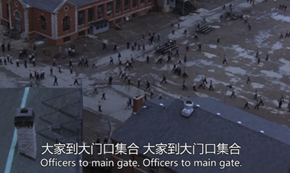
\includegraphics[scale=1.2]{./Chapter1/Figures/figure-film-subtitles.jpg}
    \caption{电影字幕}
    \label{fig:1-13}
\end{figure}
%-------------------------------------------

\parinterval (四)社交

\parinterval 社交是人们的重要社会活动。人们可以通过各种各样的社交软件做到即时通讯,进行协作或者分享自己的观点。然而受限于语言问题,人们的社交范围往往不会超出自己所掌握的语种范围,很难方便地进行跨语言社交。随着机器翻译技术的发展,越来越多的社交软件开始支持自动翻译,用户可以轻易地将各种语言的内容翻译成自己的母语,方便了人们的交流,让语言问题不再成为社交的障碍。

\parinterval (五)同声传译

\parinterval 在一些国际会议中,与会者来自许多不同的国家,为了保证会议的流畅,通常需要专业译员进行同声传译。同声传译需要在不打断演讲的同时,不间断的将讲话内容进行口译,对翻译人员的素质要求极高,成本高昂。现在,一些会议开始采用语音识别来将语音转换成文本,同时使用机器翻译技术进行翻译的方式,达到同步翻译的目的。这项技术已经得到了多个企业的关注,并在很多重要会议上进行尝试,取得了很好的反响。不过同声传译达到真正的使用还需一定时间的打磨,特别是会议场景下,准确进行语音识别和翻译仍然具有一定挑战。

\parinterval (六)医药领域翻译

\parinterval 在医药领域中,从药品研发、临床试验到药品注册,都有着大量的翻译需求。比如,在新药注册阶段,限定申报时间的同时,更是对翻译质量有着极高的要求。由于医药领域专业词汇量庞大、单词冗长复杂、术语准确且文体专业性强,翻译难度明显高于其他领域,人工翻译的方式代价大且很难满足效率的要求。为此,机器翻译近几年在医药领域取得广泛应用。在针对医药领域进行优化后,机器翻译质量可以很好地满足翻译的要求。

\parinterval (七)中国传统语言文化的翻译

\parinterval 中国几千年的历史留下了极为宝贵的文化遗产,而其中,文言文作为古代书面语,具有言文分离、行文简练的特点,易于流传。由于其言文分离的特点,使得文言文和现在的标准汉语具有一定的区别,为了更好发扬中国传统文化,需要对文言文进行翻译。而文言文古奥难懂,需要人们具备一定的文言文知识背景,否则很难准确翻译,机器翻译技术也可以帮助人们快速完成文言文的翻译。除此之外,机器翻译技术同样可以用于古诗生成和对联生成等任务。

\parinterval (八)全球化

\parinterval 在经济全球化的今天,很多企业都有国际化的需求,企业员工或多或少地会遇到一些跨语言阅读和交流的情况,比如阅读进口产品的说明书,跨国公司之间的邮件、说明文件等等。相比于成本较高的人工翻译,机器翻译往往是一种很好的选择。在一些质量要求不高的翻译场景中,机器翻译可以得到应用。

\parinterval (九)翻译机

\parinterval 出于商务、学术交流或者旅游的目的,人们在出国时会面临着跨语言交流的问题。近几年,随着出境人数的增加,不少企业推出了翻译机产品。通过结合机器翻译、语音识别和图像识别技术,翻译机实现了图像翻译和语音翻译的功能。用户可以很便捷地获取一些外语图像文字和语音信息,同时可以通过翻译机进行对话,降低跨语言交流门槛。

\parinterval (十)翻译结果后编辑

\parinterval 翻译结果后编辑是指在机器翻译的结果之上,通过少量的人工编辑来进一步完善机器译文。在传统的人工翻译过程中,翻译人员完全依靠人工的方式进行翻译,这虽然保证了翻译质量,但是时间成本高。相对应的,机器翻译具有速度快和成本低的优势。在一些领域,目前的机器翻译质量已经可以很大程度上减小翻译人员的工作量,翻译人员可以在机器翻译的辅助下,花费相对较小的代价来完成翻译。

%----------------------------------------------------------------------------------------
%    NEW SECTION
%----------------------------------------------------------------------------------------

\sectionnewpage
\section{开源项目与评测}

\parinterval 从实践的角度,机器翻译的发展主要可以归功于两方面的推动作用:开源系统和评测。开源系统通过代码共享的方式使得最新的研究成果可以快速传播,同时实验结果可以复现。而评测比赛,使得各个研究组织的成果可以进行科学的对比,共同推动机器翻译的发展与进步。此外,开源项目也促进了不同团队之间的协作,让研究人员在同一个平台上集中力量攻关。

%----------------------------------------------------------------------------------------
%    NEW SUB-SECTION
%----------------------------------------------------------------------------------------

\subsection{开源机器翻译系统}


下面列举一些优秀的开源机器翻译系统:

%----------------------------------------------------------------------------------------
%    NEW SUBSUB-SECTION
%----------------------------------------------------------------------------------------

\subsubsection{统计机器翻译开源系统}

\begin{itemize}
\vspace{0.5em}
\item NiuTrans.SMT:NiuTrans\cite{Tong2012NiuTrans}是由东北大学自然语言处理实验室自主研发的统计机器翻译系统,该系统可支持基于短语的模型、基于层次短语的模型以及基于句法的模型。由于使用C++ 语言开发,所以该系统运行时间快,所占存储空间少。系统中内嵌有$n$-gram语言模型,故无需使用其他的系统即可对完成语言建模。网址:\url{http://opensource.niutrans.com/smt/index.html}
\vspace{0.5em}
\item Moses:Moses\cite{Koehn2007Moses}是统计机器翻译时代最著名的系统之一,(主要)由爱丁堡大学的机器翻译团队开发。最新的Moses系统支持很多的功能,例如,它既支持基于短语的模型,也支持基于句法的模型。Moses 提供因子化翻译模型(Factored Translation Model),因此该模型可以很容易地对不同层次的信息进行建模。此外,它允许将混淆网络和字格作为输入,可缓解系统的1-best输出中的错误。Moses还提供了很多有用的脚本和工具,被机器翻译研究者广泛使用。网址:\url{http://www.statmt.org/moses/}
\vspace{0.5em}
\item Joshua:Joshua\cite{Li2010Joshua}是由约翰霍普金斯大学的语言和语音处理中心开发的层次短语翻译系统。由于Joshua是由Java语言开发,所以它在不同的平台上运行或开发时具有良好的可扩展性和可移植性。Joshua也是使用非常广泛的开源器翻译系统之一。网址:\url{http://joshua.sourceforge.net/Joshua/Welcome.html}
\vspace{0.5em}
\item SilkRoad:SilkRoad是由五个国内机构(中科院计算所、中科院软件所、中科院自动化所、厦门大学和哈尔滨工业大学)联合开发的基于短语的统计机器翻译系统。该系统是中国乃至亚洲地区第一个开源的统计机器翻译系统。SilkRoad支持多种解码器和规则提取模块,这样可以组合成不同的系统,提供多样的选择。网址:\url{http://www.nlp.org.cn/project/project.php?projid=14}
\vspace{0.5em}
\item SAMT:SAMT\cite{zollmann2007the}是由卡内基梅隆大学机器翻译团队开发的语法增强的统计机器翻译系统。SAMT在解码的时候使用目标树来生成翻译规则,而不严格遵守目标语言的语法。SAMT 的一个亮点是它提供了简单但高效的方式在机器翻译中使用句法信息。由于SAMT在hadoop中实现,它可受益于大数据集的分布式处理。网址:\url{http://www.cs.cmu.edu/zollmann/samt/}
\vspace{0.5em}
\item HiFST:HiFST\cite{iglesias2009hierarchical}是剑桥大学开发的统计机器翻译系统。该系统完全基于有限状态自动机实现,因此非常适合对搜索空间进行有效的表示。网址:\url{http://ucam-smt.github.io/}
\vspace{0.5em}
\item cdec:cdec\cite{dyer2010cdec}是一个强大的解码器,是由Chris Dyer 和他的合作者们一起开发。cdec的主要功能是它使用了翻译模型的一个统一的内部表示,并为结构预测问题的各种模型和算法提供了实现框架。所以,cdec也可以在被用来做一个对齐系统或者一个更通用的学习框架。此外,由于使用C++语言编写,cdec的运行速度较快。网址:\url{http://cdec-decoder.org/index.php?title=MainPage}
\vspace{0.5em}
\item Phrasal:Phrasal\cite{Cer2010Phrasal}是由斯坦福大学自然语言处理小组开发的系统。除了传统的基于短语的模型,Phrasal还支持基于非层次短语的模型,这种模型将基于短语的翻译延伸到非连续的短语翻译,增加了模型的泛化能力。网址:\url{http://nlp.stanford.edu/phrasal/}
\vspace{0.5em}
\item Jane:Jane\cite{vilar2012jane}是一个基于短语和基于层次短语的机器翻译系统,由亚琛工业大学的人类语言技术与模式识别小组开发。Jane提供了系统融合模块,因此可以非常方便的对多个系统进行融合。网址:\url{https://www-i6.informatik.rwth-aachen.de/jane/}
\vspace{0.5em}
\item GIZA++:GIZA++\cite{och2003systematic}是Franz Och研发的用于训练IBM模型1-5和HMM单词对齐模型的工具包。在早期,GIZA++是所有统计机器翻译系统中词对齐的标配工具。网址:\url{https://github.com/moses-smt/giza-pp}
\vspace{0.5em}
\item FastAlign:FastAlign\cite{dyer2013a}是一个快速,无监督的词对齐工具,由卡内基梅隆大学开发。网址:\url{https://github.com/clab/fast\_align}
\vspace{0.5em}
\end{itemize}

%----------------------------------------------------------------------------------------
%    NEW SUBSUB-SECTION
%----------------------------------------------------------------------------------------

\subsubsection{神经机器翻译开源系统}

\begin{itemize}
\vspace{0.5em}
\item GroundHog:GroundHog\cite{bahdanau2014neural}基于Theano\cite{al2016theano}框架,由蒙特利尔大学LISA 实验室使用Python语言编写的一个框架,旨在提供灵活而高效的方式来实现复杂的循环神经网络模型。它提供了包括LSTM在内的多种模型。Bahdanau等人在此框架上又编写了GroundHog神经机器翻译系统。该系统也作为了很多论文的基线系统。网址:\url{https://github.com/lisa-groundhog/GroundHog}
\vspace{0.5em}
\item Nematus:Nematus\cite{DBLP:journals/corr/SennrichFCBHHJL17}是英国爱丁堡大学开发的,基于Theano框架的神经机器翻译系统。该系统使用GRU作为隐层单元,支持多层网络。Nematus 编码端有正向和反向的编码方式,可以同时提取源语句子中的上下文信息。该系统的一个优点是,它可以支持输入端有多个特征的输入(例如词的词性等)。网址:\url{https://github.com/EdinburghNLP/nematus}
\vspace{0.5em}
\item ZophRNN:ZophRNN\cite{zoph2016simple}是由南加州大学的Barret Zoph 等人使用C++语言开发的系统。Zoph既可以训练序列表示模型(如语言模型),也可以训练序列到序列的模型(如神经机器翻译模型)。当训练神经机器翻译系统时,ZophRNN也支持多源输入。网址:\url{https://github.com/isi-nlp/Zoph\_RNN}
\vspace{0.5em}
\item Fairseq:Fairseq\cite{Ottfairseq}是由Facebook开发的,基于PyTorch框架的用以解决序列到序列问题的工具包,其中包括基于卷积神经网络、基于循环神经网络、基于Transformer的模型等。Fairseq是当今使用最广泛的神经机器翻译开源系统之一。https://github.com/facebookresearch/fairseq
\vspace{0.5em}
\item Tensor2Tensor:Tensor2Tensor\cite{VaswaniTensor2Tensor}是由谷歌推出的,基于TensorFlow框架的开源系统。该系统基于Transformer模型,因此可以支持大多数序列到序列任务。得益于Transformer 的网络结构,系统的训练速度较快。现在,Tensor2Tensor也是机器翻译领域广泛使用的开源系统之一。网址:\url{https://github.com/tensorflow/tensor2tensor}
\vspace{0.5em}
\item OpenNMT:OpenNMT\cite{KleinOpenNMT}系统是由哈佛大学自然语言处理研究组开源的,基于Torch框架的神经机器翻译系统。OpenNMT系统的早期版本使用Lua 语言编写,现在也扩展到了TensorFlow和PyTorch,设计简单易用,易于扩展,同时保持效率和翻译精度。网址:\url{https://github.com/OpenNMT/OpenNMT}
\vspace{0.5em}
\item 斯坦福神经机器翻译开源代码库:斯坦福大学自然语言处理组(Stanford NLP)发布了一篇教程,介绍了该研究组在神经机器翻译上的研究信息,同时实现了多种翻译模型\cite{luong2016acl_hybrid}。 网址:\url{https://nlp.stanford.edu/projects/nmt/}
\vspace{0.5em}
\item THUMT:清华大学NLP团队实现的神经机器翻译系统,支持Transformer等模型\cite{ZhangTHUMT}。该系统主要基于Tensorflow和Theano实现,其中Theano版本包含了RNNsearch模型,训练方式包括MLE (Maximum Likelihood Estimate), MRT\\(Minimum Risk Training), SST(Semi-Supervised Training)。Tensorflow 版本实现了Seq2Seq, RNNsearch, Transformer三种基本模型。网址:\url{https://github.com/THUNLP-MT/THUMT}
\vspace{0.5em}
\item NiuTrans.NMT:由小牛翻译团队基于NiuTensor实现的神经机器翻译系统。支持循环神经网络、Transformer等结构,并支持语言建模、序列标注、机器翻译等任务。支持机器翻译GPU与CPU 训练及解码。其小巧易用,为开发人员提供快速二次开发基础。此外,NiuTrans.NMT已经得到了大规模应用,形成了支持187种语言翻译的小牛翻译系统。网址:\url{http://opensource.niutrans.com/niutensor/index.html}
\vspace{0.5em}
\item MARIAN:主要由微软翻译团队搭建\cite{JunczysMarian},其使用C++实现的用于GPU/CPU训练和解码的引擎,支持多GPU训练和批量解码,最小限度依赖第三方库,静态编译一次之后,复制其二进制文件就能在其他平台使用。网址:\url{https://marian-nmt.github.io/}
\vspace{0.5em}
\item Sockeye:由Awslabs开发的神经机器翻译框架\cite{hieber2017sockeye}。其中支持RNNSearch、Transformer、CNN等翻译模型,同时提供了从图片翻译到文字的模块以及WMT 德英新闻翻译、领域适应任务、多语言零资源翻译任务的教程。网址:\url{https://awslabs.github.io/sockeye/}
\vspace{0.5em}
\item CytonMT:由NICT开发的一种用C++实现的神经机器翻译开源工具包\cite{WangCytonMT}。主要支持Transformer模型,并支持一些常用的训练方法以及解码方法。网址:\url{https://github.com/arthurxlw/cytonMt}
\vspace{0.5em}
\item OpenSeq2Seq:由NVIDIA团队开发的\cite{DBLP:journals/corr/abs-1805-10387}基于Tensorflow的模块化架构,用于序列到序列的模型,允许从可用组件中组装新模型,支持混合精度训练,利用NVIDIA Volta Turing GPU中的Tensor核心,基于Horovod的快速分布式训练,支持多GPU,多节点多模式。网址:\url{https://nvidia.github.io/OpenSeq2Seq/html/index.html}
\vspace{0.5em}
\item NMTPyTorch:由勒芒大学语言实验室发布的基于序列到序列框架的神经网络翻译系统\cite{nmtpy2017},Nmtpytorch的核心部分依赖于Numpy,Pytorch和tqdm。其允许训练各种端到端神经体系结构,包括但不限于神经机器翻译,图像字幕和自动语音识别系统。网址:\url{https://github.com/lium-lst/nmtpytorch}
\vspace{0.5em}
\end{itemize}


%----------------------------------------------------------------------------------------
%    NEW SUB-SECTION
%----------------------------------------------------------------------------------------

\subsection{常用数据集及公开评测任务}

\parinterval 机器翻译相关评测主要有两种组织形式,一种是由政府及国家相关机构组织,权威性强。如由美国国家标准技术研究所组织的NIST评测、日本国家科学咨询系统中心主办的NACSIS Test Collections for IR(NTCIR)PatentMT、日本科学振兴机构(Japan Science and Technology Agency,简称JST)等组织联合举办的Workshop on Asian Translation(WAT)以及国内由中文信息学会主办的全国机器翻译大会(China Conference on Machine Translation,简称CCMT);另一种是由相关学术机构组织,具有领域针对性的特点,如倾向新闻领域的Workshop on Statistical Machine Translation(WMT)以及面向口语的International Workshop on Spoken Language Translation(IWSLT)。下面将针对上述评测进行简要介绍。

\begin{itemize}
\vspace{0.5em}
\item CCMT(全国机器翻译大会),前身为CWMT(全国机器翻译研讨会)是国内机器翻译领域的旗舰会议,自2005年起已经组织多次机器翻译评测,对国内机器翻译相关技术的发展产生了深远影响。该评测主要针对汉语、英语以及国内的少数民族语言(蒙古语、藏语、维吾尔语等)进行评测,领域包括新闻、口语、政府文件等,不同语言方向对应的领域也有所不同。评价方式不同届略有不同,主要采用自动评价的方式,自CWMT 2013起则针对某些领域增设人工评价。自动评价的指标一般包括BLEU-SBP、BLEU-NIST、TER、METEOR、NIST、GTM、mWER、mPER 以及ICT 等,其中以BLEU-SBP 为主,汉语为目标语的翻译采用基于字符的评价方式,面向英语的翻译采用基于词的评价方式。每年该评测吸引国内外近数十家企业及科研机构参赛,业内认可度极高。关于CCMT的更多信息可参考官网:\url{http://www.ai-ia.ac.cn/cwmt2015/evaluation.html} (链接为CWMT 2015)。
\vspace{0.5em}
\item WMT由Special Interest Group for Machine Translation(SIGMT)主办,会议自2006年起每年召开一次,是一个涉及机器翻译多种任务的综合性会议,包括多领域翻译评测任务、质量评价任务以及其他与机器翻译的相关任务(如文档对齐评测等)。现在WMT已经成为机器翻译领域的旗舰评测任务,很多研究工作都以WMT任务作为基准。WMT评测涉及的语言范围较广,包括英语、德语、芬兰语、捷克语、罗马尼亚语等十多种语言,翻译方向一般以英语为核心,探索英语与其他语言之间的翻译性能,领域包括新闻、信息技术、生物医学。最近,也增加了无指导机器翻译等热门问题。WMT在评价方面类似于CCMT,也采用人工评价与自动评价相结合的方式,自动评价的指标一般为BLEU、TER 等。此外,WMT公开了所有评测数据,因此也经常被机器翻译相关人员所使用。更多WMT的机器翻译评测相关信息可参考官网:\url{http://www.sigmt.org/}。
\vspace{0.5em}
\item NIST机器翻译评测开始于2001年,是早期机器翻译公开评测中颇具代表性的任务,现在WMT和CCMT很多任务的设置也大量参考了当年NIST评测的内容。NIST评测由美国国家标准技术研究所主办,作为美国国防高级计划署(DARPA)中TIDES计划的重要组成部分。早期,NIST评测主要评价阿拉伯语和汉语等语言到英语的翻译效果,评价方法一般采用人工评价与自动评价相结合的方式。人工评价采用5分制评价。自动评价使用多种方式,包括BLEU,METEOR,TER以及HyTER。此外NIST从2016 年起开始对稀缺语言资源技术进行评估,其中机器翻译作为其重要组成部分共同参与评测,评测指标主要为BLEU。除对机器翻译系统进行评测之外,NIST在2008 和2010年对于机器翻译的自动评价方法(MetricsMaTr)也进行了评估,以鼓励更多研究人员对现有评价方法进行改进或提出更加贴合人工评价的方法。同时NIST评测所提供的数据集由于数据质量较高受到众多科研人员喜爱,如MT04,MT06等(汉英)平行语料经常被科研人员在实验中使用。不过,近几年NIST评测已经停止。更多NIST的机器翻译评测相关信息可参考官网:\url{https://www.nist.gov/programs-projects/machine-translation}。
\vspace{0.5em}
\item 从2004年开始举办的IWSLT也是颇具特色的机器翻译评测,它主要关注口语相关的机器翻译任务,测试数据包括TED talks的多语言字幕以及QED 教育讲座影片字幕等,语言涉及英语、法语、德语、捷克语、汉语、阿拉伯语等众多语言。此外在IWSLT 2016 中还加入了对于日常对话的翻译评测,尝试将微软Skype中一种语言的对话翻译成其他语言。评价方式采用自动评价的模式,评价标准和WMT类似,一般为BLEU 等指标。另外,IWSLT除了对文本到文本的翻译评测外,还有自动语音识别以及语音转另一种语言的文本的评测。更多IWSLT的机器翻译评测相关信息可参考官网:\url{https://workshop2016.iwslt.org/} (链接为IWSLT2016)
\vspace{0.5em}
\item 日本举办的机器翻译评测WAT是亚洲范围内的重要评测之一,由日本科学振兴机构(JST)、情报通信研究机构(NICT)等多家机构共同组织,旨在为亚洲各国之间交流融合提供便宜之处。语言方向主要包括亚洲主流语言(汉语、韩语、印地语等)以及英语对日语的翻译,领域丰富多样,包括学术论文、专利、新闻、食谱等。评价方式包括自动评价(BLEU、RIBES以及AMFM 等)以及人工评价,其特点在于对于测试语料以段落为单位进行评价,考察其上下文关联的翻译效果。更多WAT的机器翻译评测相关信息可参考官网:\url{http://lotus.kuee.kyoto-u.ac.jp/WAT/}。
\vspace{0.5em}
\item NTCIR计划是由日本国家科学咨询系统中心策划主办的,旨在建立一个用在自然语言处理以及信息检索相关任务上的日文标准测试集。在NTCIR-9的和NTCIR-10中开设的Patent Machine Translation(PatentMT)任务主要针对专利领域进行翻译测试,其目的在于促进机器翻译在专利领域的发展和应用。在NTCIR-9中,评测方式采取人工评价与自动评价相结合,以人工评价为主导。人工评价主要根据准确度和流畅度进行评估,自动评价采用BLEU、NIST等方式进行。NTCIR-10评价方式在此基础上增加了专利审查评估、时间评估以及多语种评估,分别考察机器翻译系统在专利领域翻译的实用性、耗时情况以及不同语种的翻译效果等。更多NTCIR评测相关信息可参考官网:\url{http://research.nii.ac.jp/ntcir/index-en.html}
\vspace{0.5em}
\end{itemize}

\parinterval 以上评测数据大多可以从评测网站上下载,此外部分数据也可以从LDC(Lingu-istic Data Consortium)上申请,网址为\url{https://www.ldc.upenn.edu/}。ELRA(Euro-pean Language Resources Association)上也有一些免费的语料库供研究使用,其官网为\url{http://www.elra.info/}。更多机器翻译的语料信息可参看附录\ref{appendix-A}。

\parinterval 从机器翻译发展的角度看,这些评测任务给相关研究提供了基准数据集,使得不同的系统都可以在同一个环境下进行比较和分析,进而建立了机器翻译研究所需的实验基础。此外,公开评测也使得研究者可以第一时间了解机器翻译研究的最新成果,比如,有多篇ACL会议最佳论文的灵感就来自当年参加机器翻译评测任务的系统。

%----------------------------------------------------------------------------------------
%    NEW SECTION
%----------------------------------------------------------------------------------------

\sectionnewpage
\section{推荐学习资源}

\parinterval 首先,推荐一本书《Statistical Machine Translation》\cite{koehn2009statistical},其作者是机器翻译领域著名学者Philipp Koehn教授。该书是机器翻译领域内的经典之作,介绍了统计机器翻译技术的进展。该书从语言学和概率学两个方面介绍了统计机器翻译的构成要素,然后介绍了统计机器翻译的主要模型:基于词、基于短语和基于树的模型,以及机器翻译评价、语言建模、判别式训练等方法。此外,作者在该书的最新版本中增加了神经机器翻译的章节,方便研究人员全面了解机器翻译的最新发展趋势\cite{DBLP:journals/corr/abs-1709-07809}。

\parinterval 《Foundations of Statistical Natural Language Processing》\cite{manning1999foundations}中文译名《统计自然语言处理基础》,作者是自然语言处理领域的权威Chris Manning教授和Hinrich Sch$\ddot{\textrm{u}}$tze教授。该书对统计自然语言处理方法进行了全面介绍。书中讲解了统计自然语言处理所需的语言学和概率论基础知识,介绍了机器翻译评价、语言建模、判别式训练以及整合语言学信息等基础方法。其中也包含了构建自然语言处理工具所需的基本理论和算法,提供了对数学和语言学基础内容广泛而严格的覆盖,以及统计方法的详细讨论。

\parinterval 《统计自然语言处理》\cite{宗成庆2013统计自然语言处理}由中国科学院自动化所宗成庆教授所著。该书中系统介绍了统计自然语言处理的基本概念、理论方法和最新研究进展,既有对基础知识和理论模型的介绍,也有对相关问题的研究背景、实现方法和技术现状的详细阐述。可供从事自然语言处理、机器翻译等研究的相关人员参考。

\parinterval  Ian Goodfellow、Yoshua Bengio,Aaron Courville三位机器学习领域的学者所写的《Deep Learning》\cite{Goodfellow-et-al-2016}也是值得一读的参考书。其讲解了有关深度学习常用的方法,其中很多都会在深度学习模型设计和使用中用到。同时在该书的应用一章中也简单讲解了神经机器翻译的任务定义和发展过程。

\parinterval 《Neural Network Methods for Natural Language Processing》\cite{goldberg2017neural}是Yoav Goldberg编写的面向自然语言处理的深度学习参考书。相比《Deep Learning》,该书聚焦在自然语言处理中的深度学习方法,内容更加易读,非常适合刚入门自然语言处理及深度学习应用的人员参考。

\parinterval 《机器学习》\cite{周志华2016机器学习}由南京大学教授周志华教授所著,作为机器学习领域入门教材,该书尽可能地涵盖了机器学习基础知识的各个方面,试图尽可能少地使用数学知识介绍机器学习方法与思想。

\parinterval 《统计学习方法》\cite{李航2012统计学习方法}由李航博士所著,该书对机器学习的有监督和无监督等方法进行了全面而系统的介绍。可以作为梳理机器学习的知识体系,同时了解相关基础概念的参考读物。

\parinterval 《神经网络与深度学习》\cite{邱锡鹏2020神经网络与深度学习}由复旦大学邱锡鹏教授所著,全面的介绍了神经网络和深度学习的基本概念和常用技术,同时涉及了许多深度学习的前沿方法。该书适合初学者阅读,同时又不失为一本面向专业人士的参考书。

\parinterval  TensorFlow官网提供了一个有关神经机器翻译的教程,介绍了从数据处理开始如何利用TensorFlow工具从零搭建一个神经机器翻译系统以及如何解码,其地址为\url{https://www.tensorflow.org/tutorials/text/nmt\_with\_attention}。此外谷歌和Facebook也分别提供了基于序列到序列机器翻译模型的高级教程。谷歌的版本是基于TensorFlow实现,网址为:\url{https://github.com/tensorflow/nmt},Facebook的教程主要是基于PyTorch实现,网址为:\url{https://pytorch.org/tutorials/intermediate/seq2seq\_translation\_tutorial.html}。网站上也包含一些综述论文,其中详细的介绍了神经机器翻译的发展历程,问题定义以及目前遇到的问题。

\parinterval  \url{http://www.statmt.org}是一个介绍机器翻译研究的网站,该网站包含了对统计机器翻译研究的一些介绍资料,一些自然语言处理的会议,常用工具以及语料库。\url{http://www.mt-archive.info}与\url{https://www.aclweb.org/anthology}\\网站上有许多介绍机器翻译和自然语言处理的论文。通过这个网站可以了解到自然语言处理领域的一些重要的期刊和会议。比如,一些与机器翻译相关的主要会议有:

\begin{itemize}
\vspace{0.5em}
\item ACL,全称Annual Meeting of the Association for Computational Linguistics,是自然语言处理领域最高级别的会议。每年举办一次,主题涵盖计算语言学的所有方向。
\vspace{0.5em}
\item NAACL,全称The North American Chapter of the Association for Computational Linguistics,为ACL北美分会,在自然语言处理领域也属于顶级会议,每年会选择一个北美城市召开会议。
\vspace{0.5em}
\item EMNLP,全称Conference on Empirical Methods in Natural Language Processing ,自然语言处理另一个顶级会议之一,由ACL当中对语言数据和经验方法有特殊兴趣的团体主办,始于1996年。会议比较偏重于方法和经验性结果。
\vspace{0.5em}
\item COLING,全称International Committee on Computational Linguistics,自然语言处理老牌顶级会议之一。该会议始于1965年,是由ICCL国际计算语言学委员会主办。会议简称为COLING,是谐音瑞典著名作家 Albert Engstr$\ddot{\textrm{o}}$m小说中的虚构人物Kolingen。COLING每两年举办一次。
\vspace{0.5em}
\item EACL,全称European Chapter of the Association for Computational Linguistics,为ACL欧洲分会,虽然在欧洲召开,会议也吸引了全世界的大量学者投稿并参会。
\vspace{0.5em}
\item AACL,全称Conference of the Asia-Pacific Chapter of the Association for Computational Linguistics,为ACL亚太地区分会。2020年会议首次召开,是亚洲地区自然语言处理领域最具影响力的会议之一。
\vspace{0.5em}
\item WMT,全称Workshop on Machine Translation。机器翻译领域一年一度研讨会,是国际公认的顶级机器翻译赛事之一。
\vspace{0.5em}
\item AMTA,全称Association for Machine Translation in the Americas。AMTA会议汇聚了学术界、产业界和政府的研究人员、开发人员和用户,让工业界和学术界进行交流。
\vspace{0.5em}
\item CCL,全称Conference on Computational Linguistics,中文为中国计算语言学大会。中国计算语言学大会创办于1991年,由中国中文信息学会计算语言学专业委员会负责组织。经过20余年的发展,中国计算语言学大会已成为国内自然语言处理领域权威性最高、规模和影响最大的学术会议。作为中国中文信息学会(国内一级学会)的旗舰会议,CCL聚焦于中国境内各类语言的智能计算和信息处理,为研讨和传播计算语言学最新学术和技术成果提供了最广泛的高层次交流平台。
\vspace{0.5em}
\item NLPCC,全称The CCF International Conference on Natural Language Processing and Chinese Computing。NLPCC 是由中国计算机学会(CCF)主办的 CCF 中文信息技术专业委员会年度学术会议,专注于自然语言处理及中文处理领域的研究和应用创新。会议自 2012 年开始举办,主要活动有主题演讲、论文报告、技术测评等多种形式。
\vspace{0.5em}
\item CCMT,全称The China Conference on Machine Translation,中国机器翻译研讨会,由中国中文信息学会主办,旨在为国内外机器翻译界同行提供一个平台,促进中国机器翻译事业。CCMT不仅是国内机器翻译领域最具影响力、最权威的学术和评测活动,而且也代表着汉语与民族语言翻译技术的最高水准,对民族语言技术发展具有重要意义。
\vspace{0.5em}
\end{itemize}

除了会议之外,《中文信息学报》、《Computational Linguistics》、《Machine Translation》、《Transactions of the Association for Computational Linguistics》、《IEEE/ACM Transactions on Audio, Speech, and Language Processing》、《ACM Transactions on Asian and Low Resource Language Information Processing》、《Natural Language Engineering》等期刊也发表了许多与机器翻译相关的重要论文。










